
\begin{frame}{analog\_vs\_digital.eps}
  \centerline{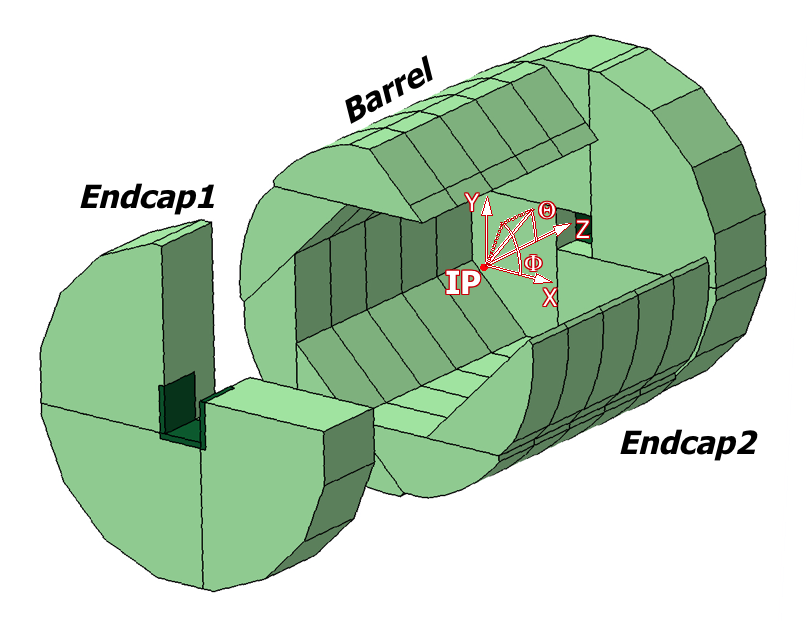
\includegraphics[width=0.9\textwidth]{images/IldDhcal}}
\end{frame}
\begin{frame}{analog\_vs\_digital.eps}
  \centerline{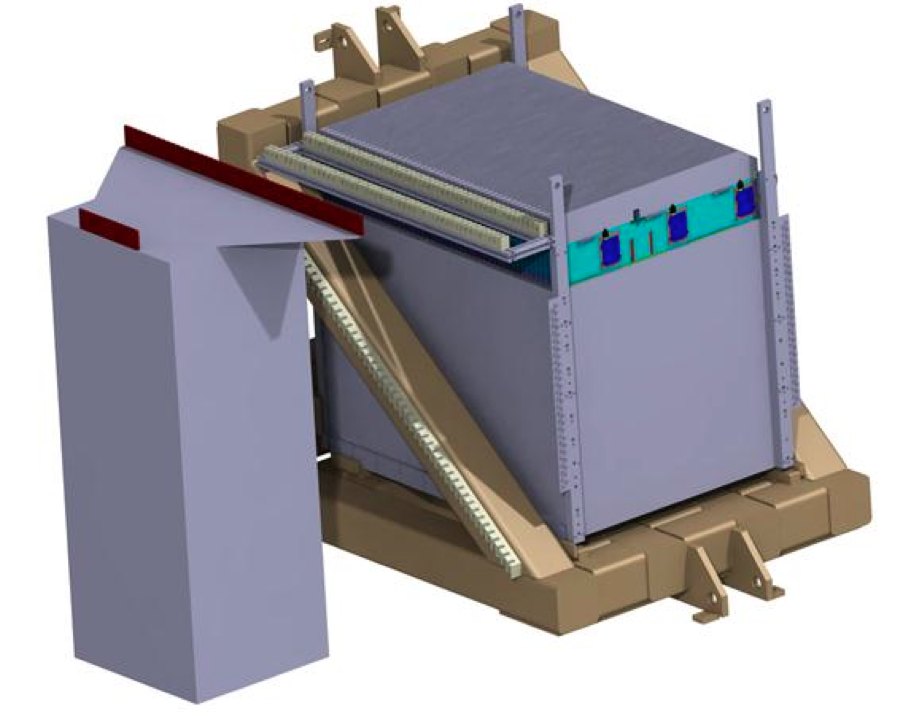
\includegraphics[width=0.9\textwidth]{images/DHCALProtoSchema}}
\end{frame}
\begin{frame}{analog\_vs\_digital.eps}
  \centerline{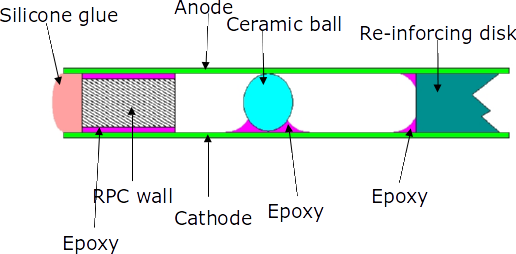
\includegraphics[width=0.9\textwidth]{images/RPCSchema}}
\end{frame}
\begin{frame}{analog\_vs\_digital.eps}
  \centerline{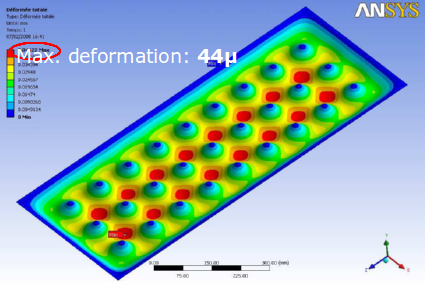
\includegraphics[width=0.9\textwidth]{images/DeformationStudies}}
\end{frame}
\begin{frame}{analog\_vs\_digital.eps}
  \centerline{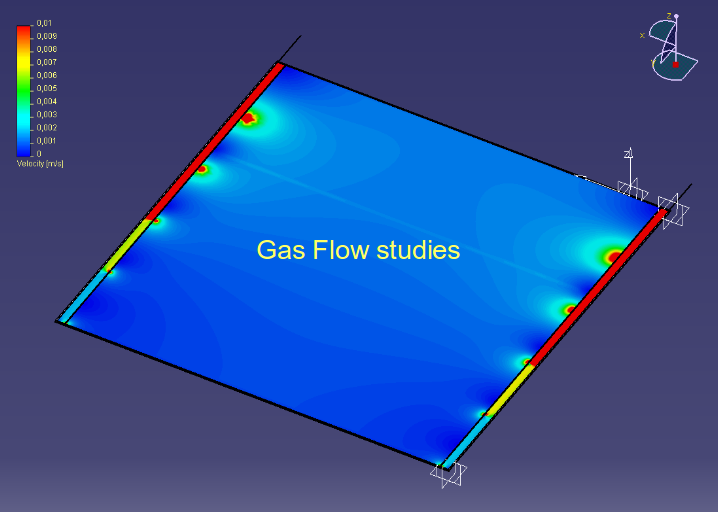
\includegraphics[width=0.9\textwidth]{images/GasFlow}}
\end{frame}
\begin{frame}{analog\_vs\_digital.eps}
  \centerline{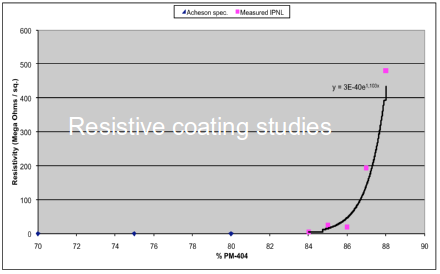
\includegraphics[width=0.9\textwidth]{images/CoatingStudies}}
\end{frame}
\begin{frame}{analog\_vs\_digital.eps}
  \centerline{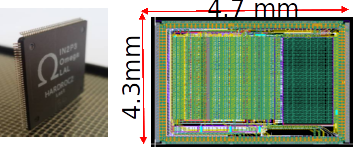
\includegraphics[width=0.9\textwidth]{images/HR2Chip}}
\end{frame}
\begin{frame}{analog\_vs\_digital.eps}
  \centerline{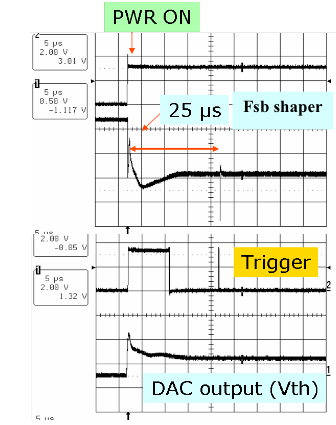
\includegraphics[width=0.9\textwidth]{images/PowerPulsingTiming}}
\end{frame}
\begin{frame}{analog\_vs\_digital.eps}
  \centerline{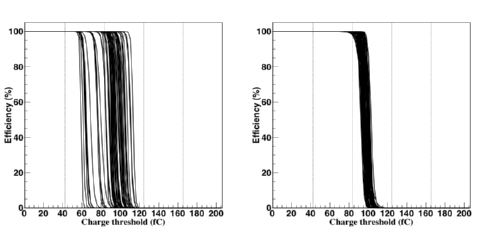
\includegraphics[width=0.9\textwidth]{images/HR2GainAdjustement}}
\end{frame}
\begin{frame}{analog\_vs\_digital.eps}
  \centerline{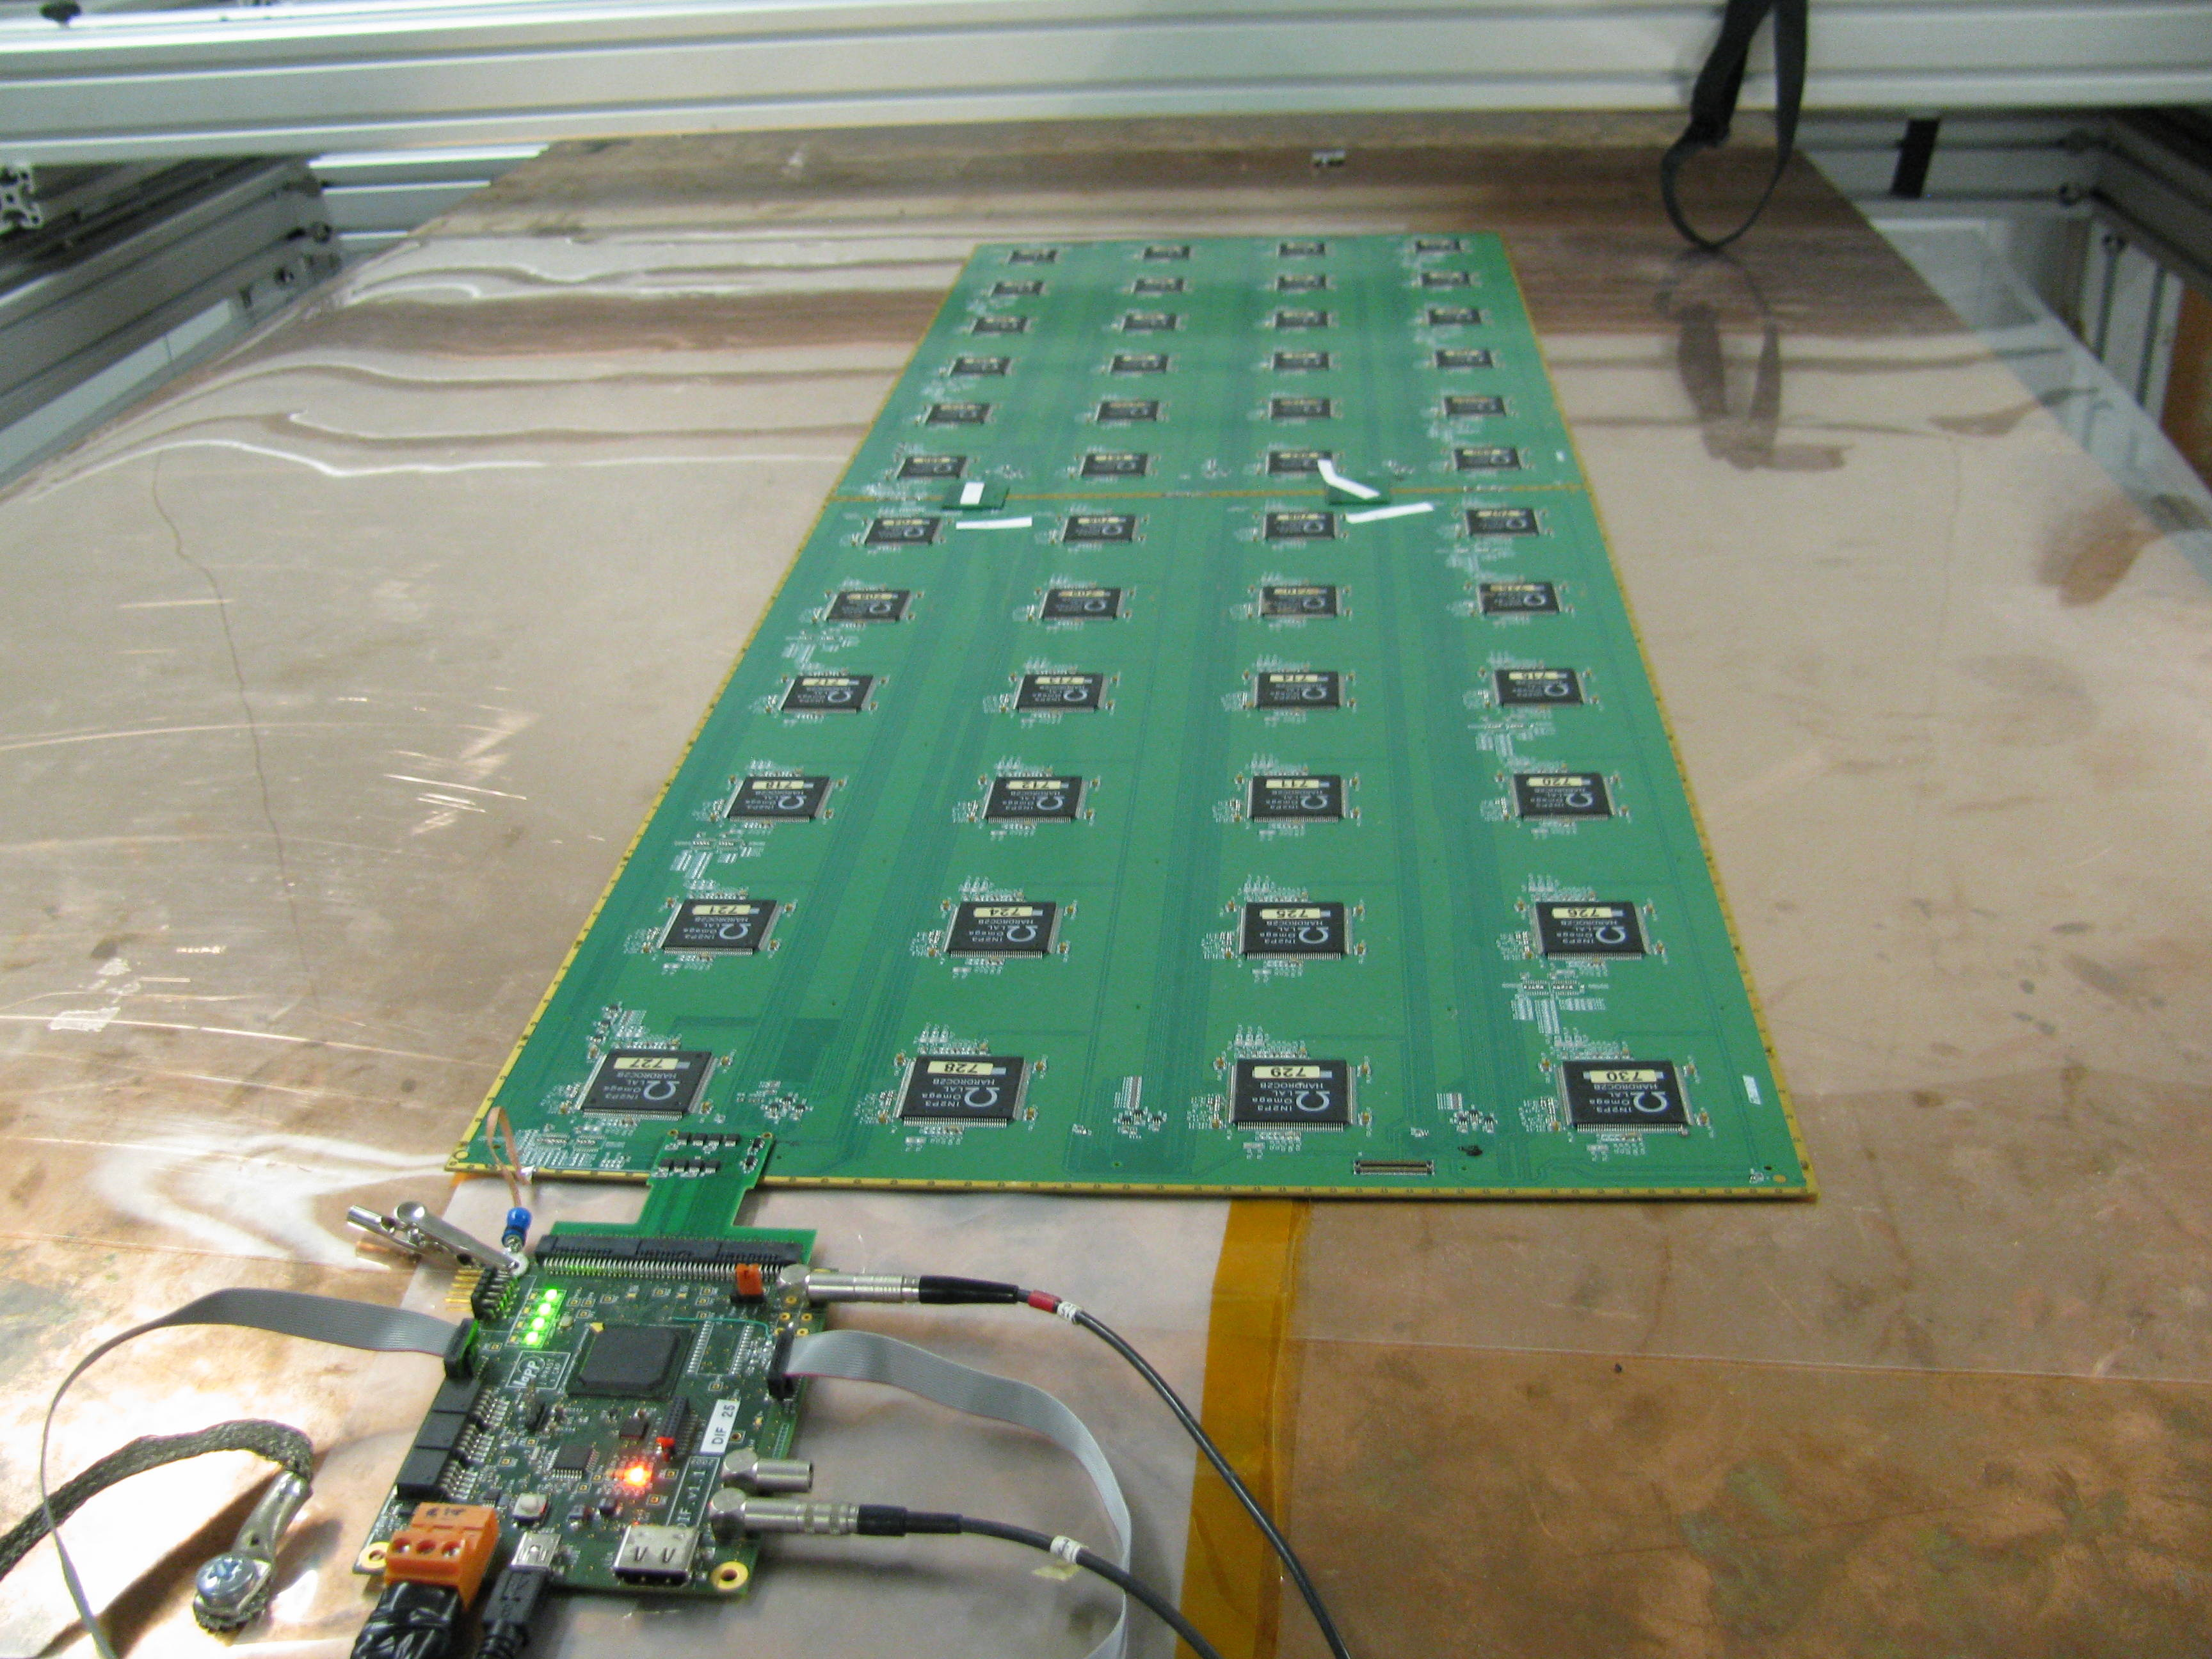
\includegraphics[width=0.9\textwidth]{images/DIFAsu}}
\end{frame}
\begin{frame}{analog\_vs\_digital.eps}
  \centerline{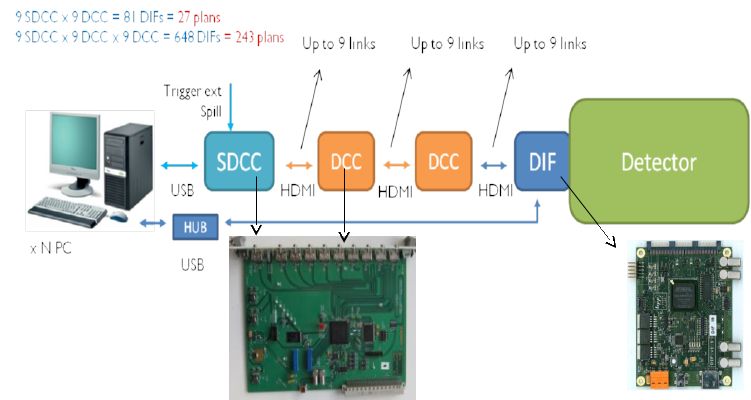
\includegraphics[width=0.9\textwidth]{images/DAQLinks}}
\end{frame}
\begin{frame}{analog\_vs\_digital.eps}
  \centerline{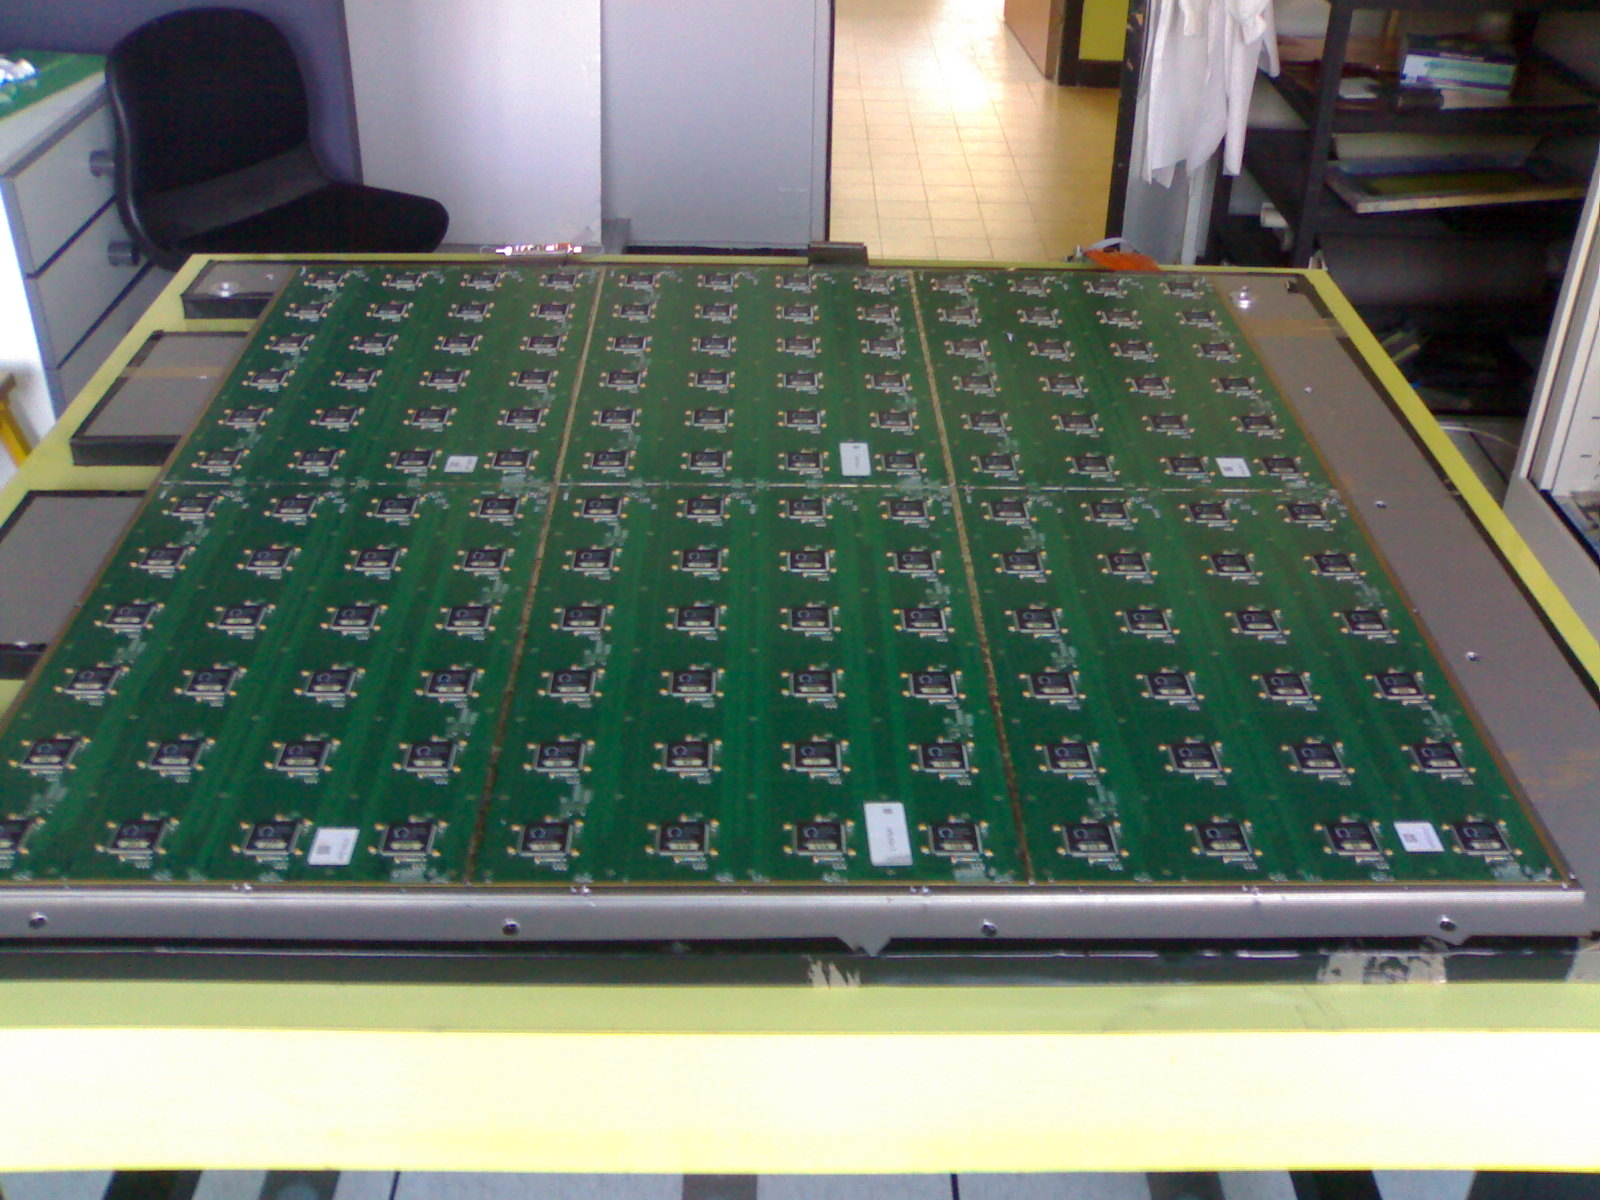
\includegraphics[width=0.9\textwidth]{images/1m2HR2}}
\end{frame}
\begin{frame}{analog\_vs\_digital.eps}
  \centerline{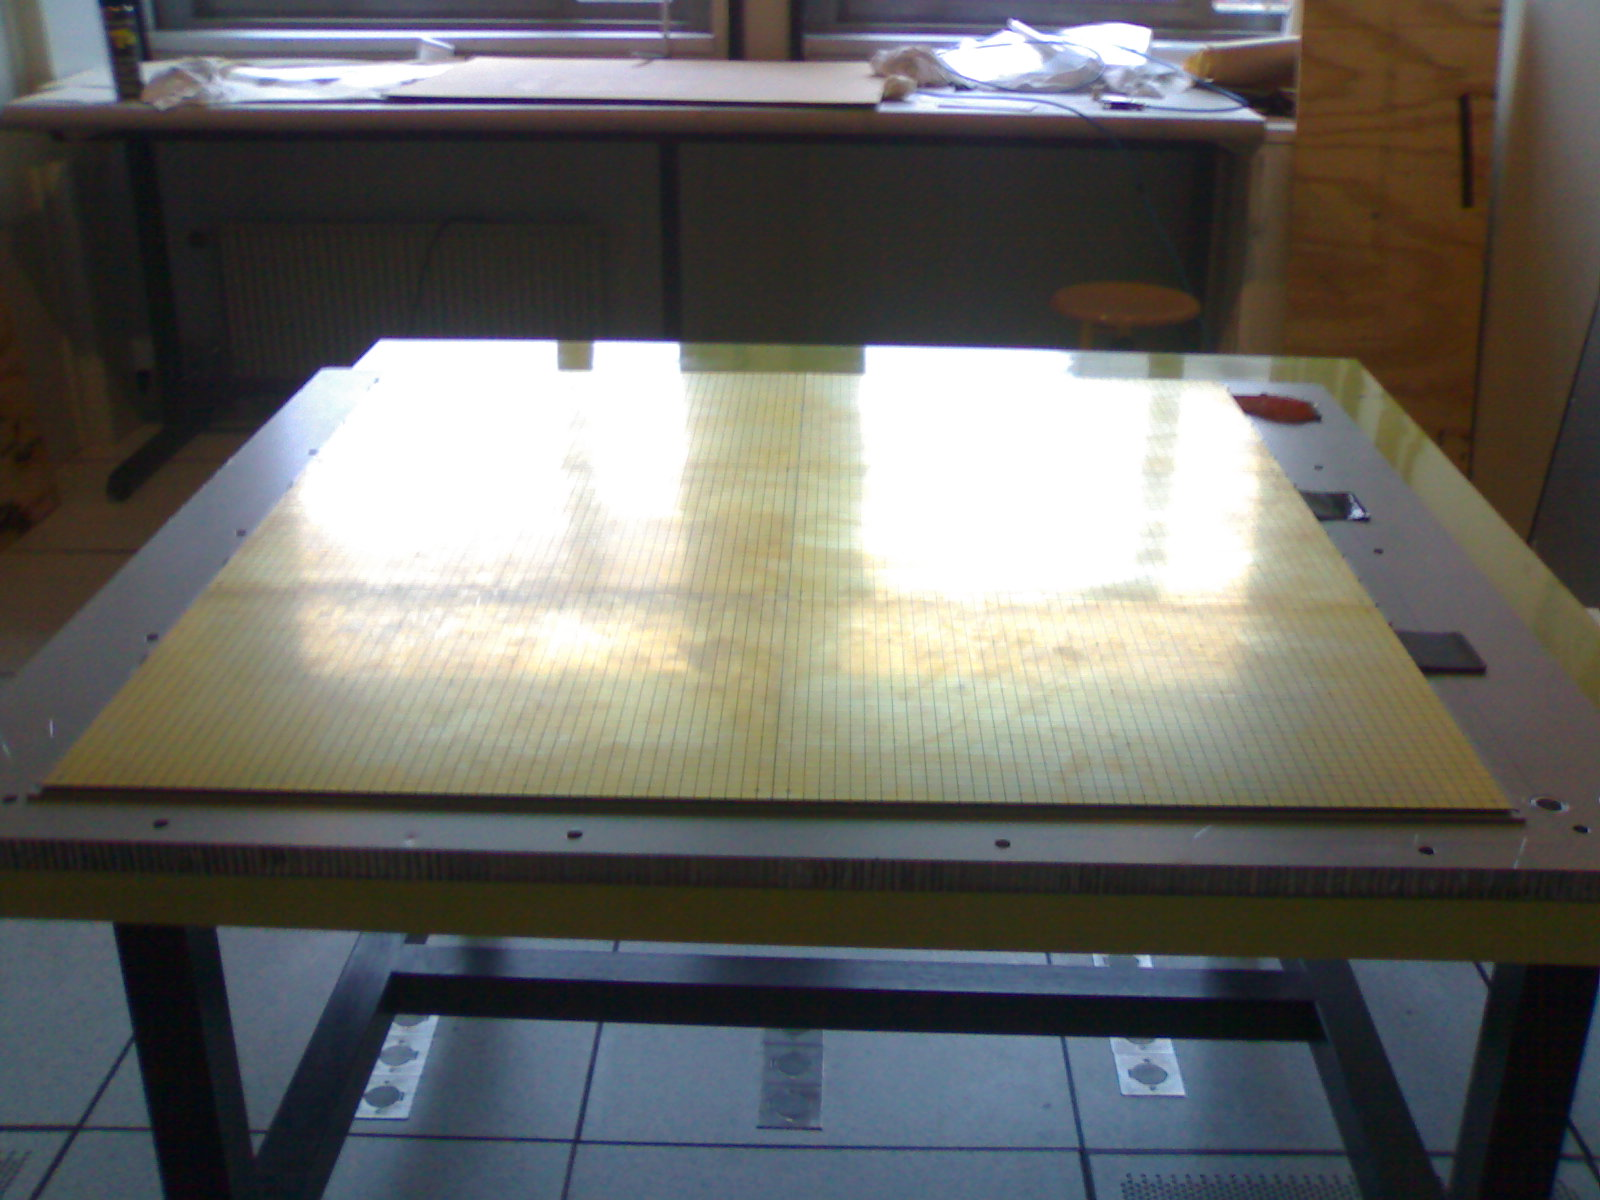
\includegraphics[width=0.9\textwidth]{images/1m2Pad}}
\end{frame}
\begin{frame}{analog\_vs\_digital.eps}
  \centerline{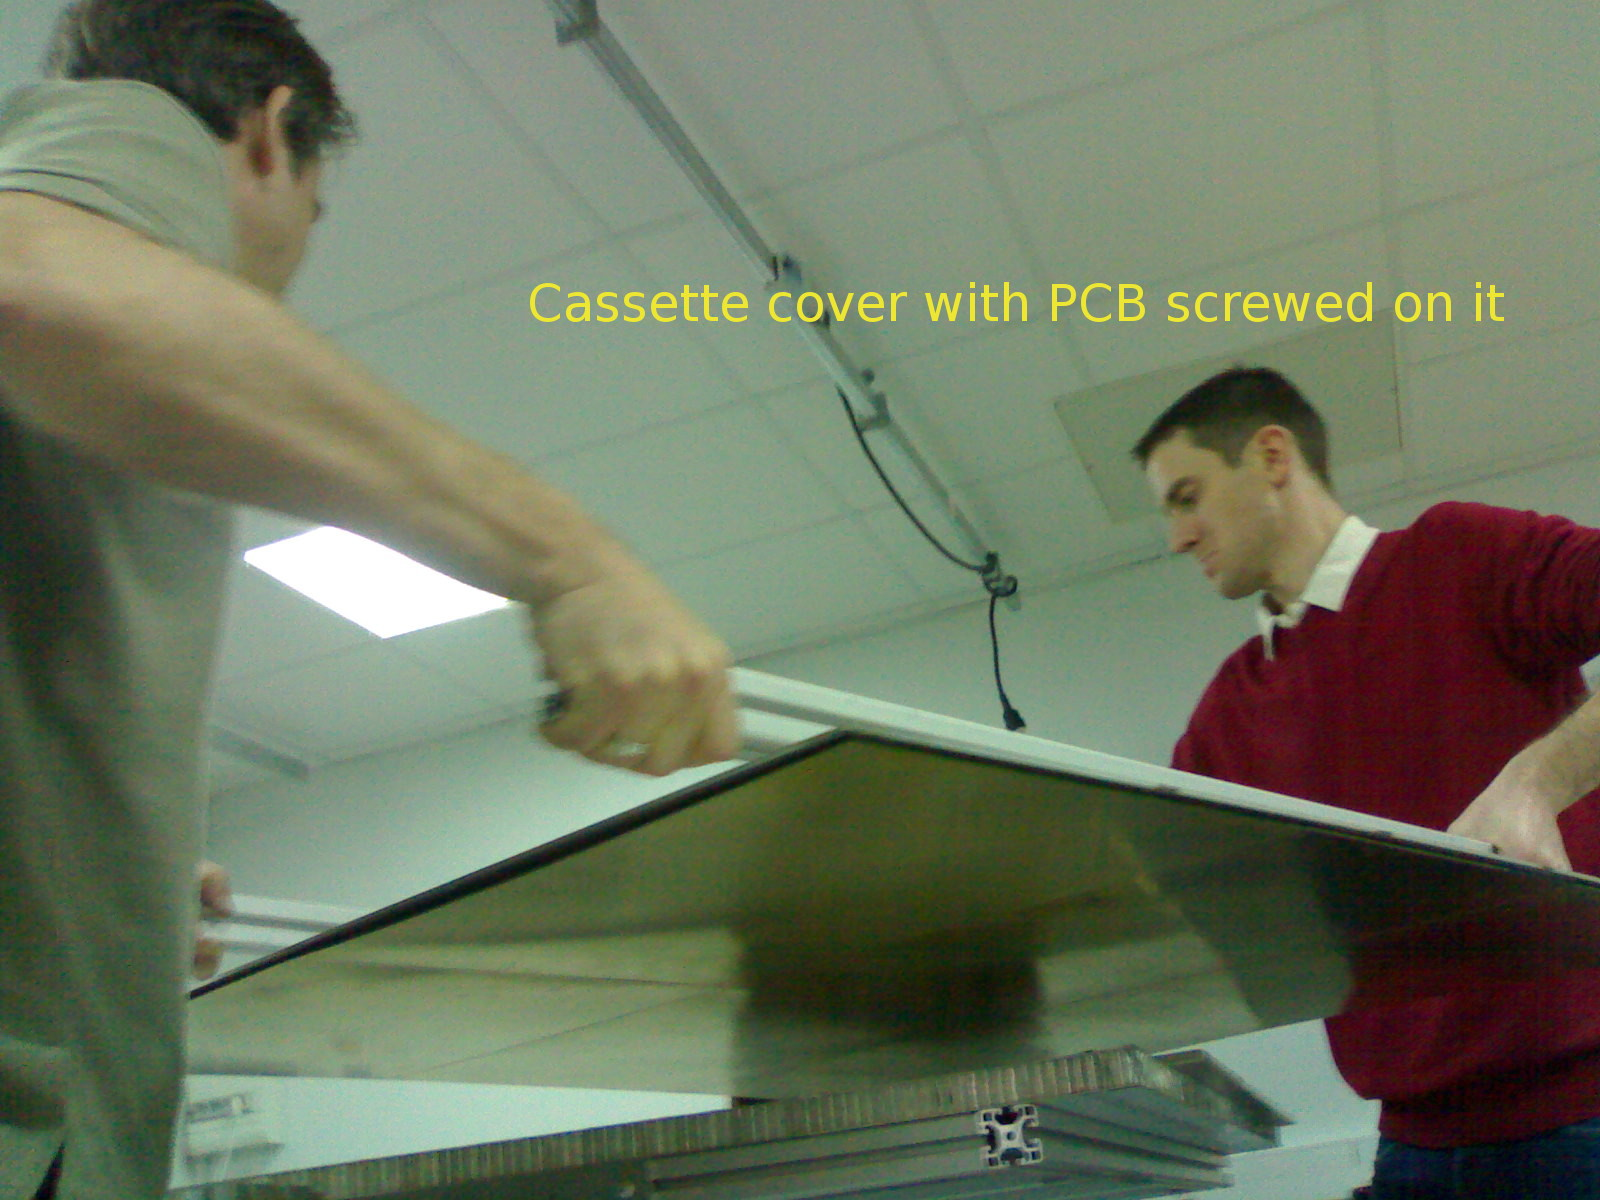
\includegraphics[width=0.9\textwidth]{images/1m2Cover}}
\end{frame}
\begin{frame}{analog\_vs\_digital.eps}
  \centerline{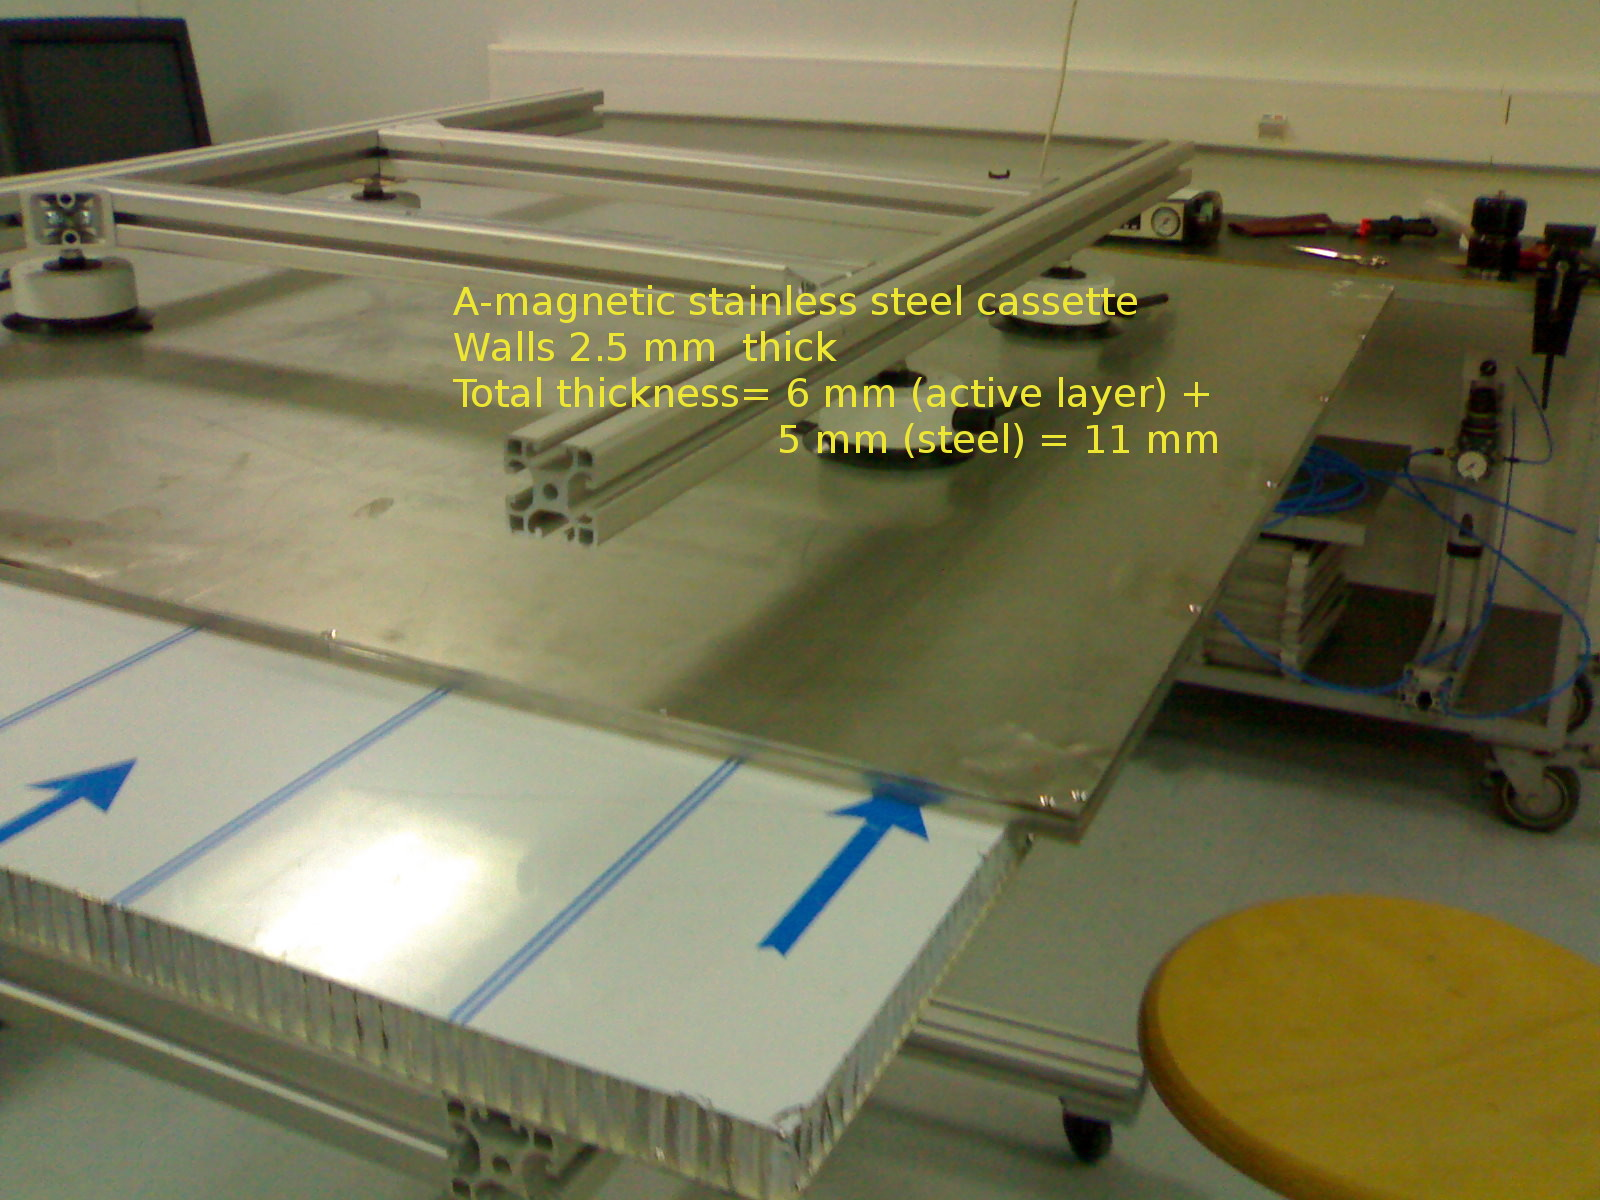
\includegraphics[width=0.9\textwidth]{images/1m2Cassette}}
\end{frame}

\begin{frame}{analog\_vs\_digital.eps}
  \centerline{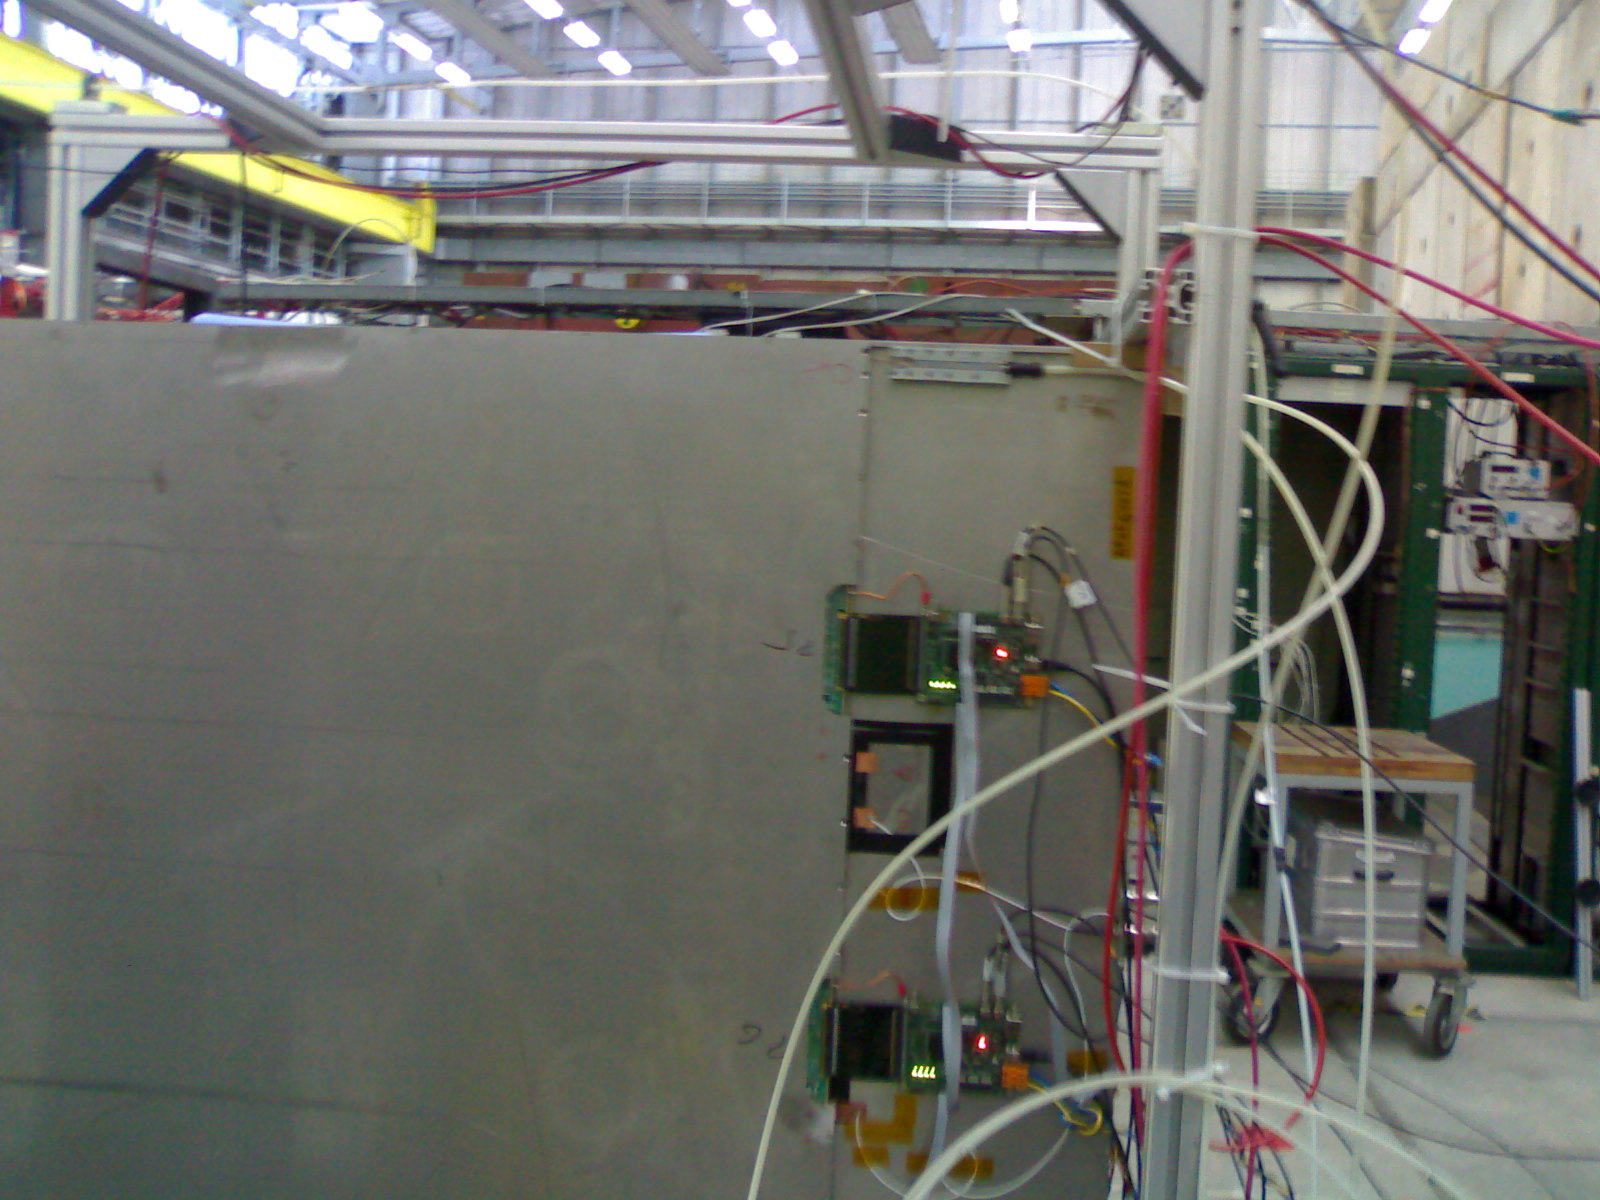
\includegraphics[width=0.9\textwidth]{images/Test1m2Photo}}
\end{frame}
\begin{frame}{analog\_vs\_digital.eps}
  \centerline{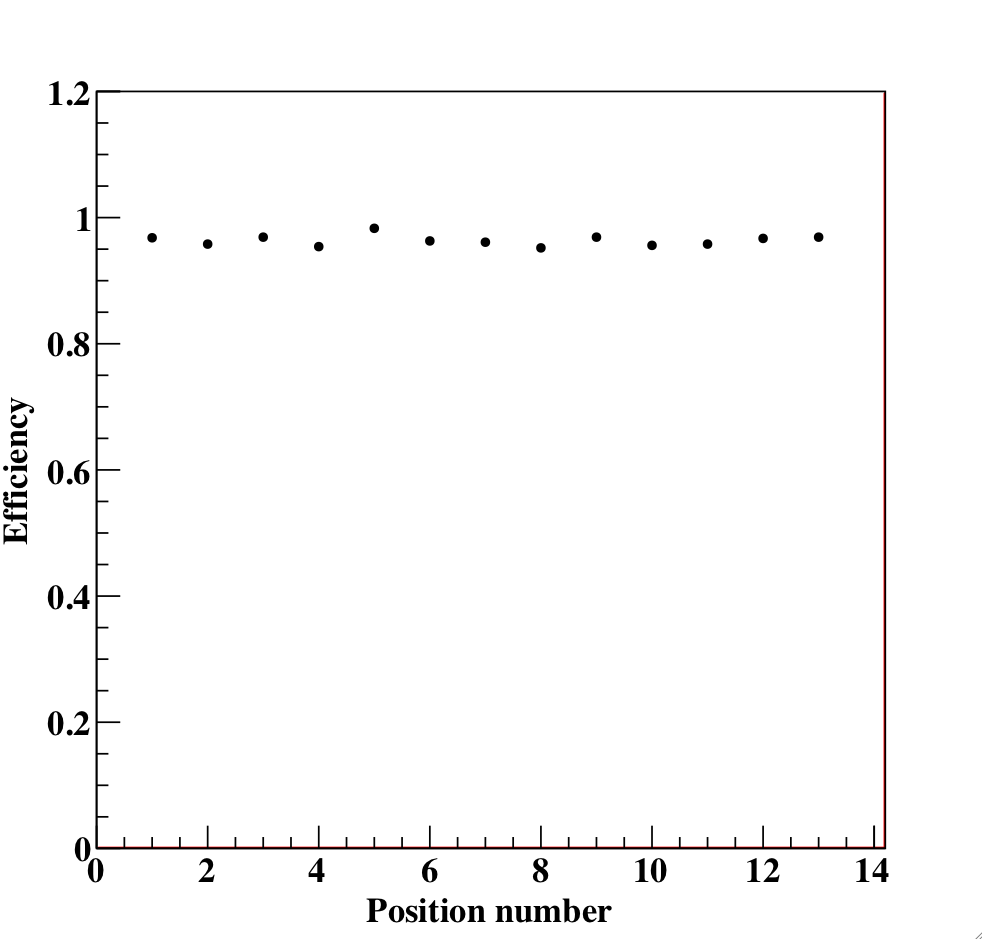
\includegraphics[width=0.9\textwidth]{images/Test1m2Efficiency}}
\end{frame}
\begin{frame}{analog\_vs\_digital.eps}
  \centerline{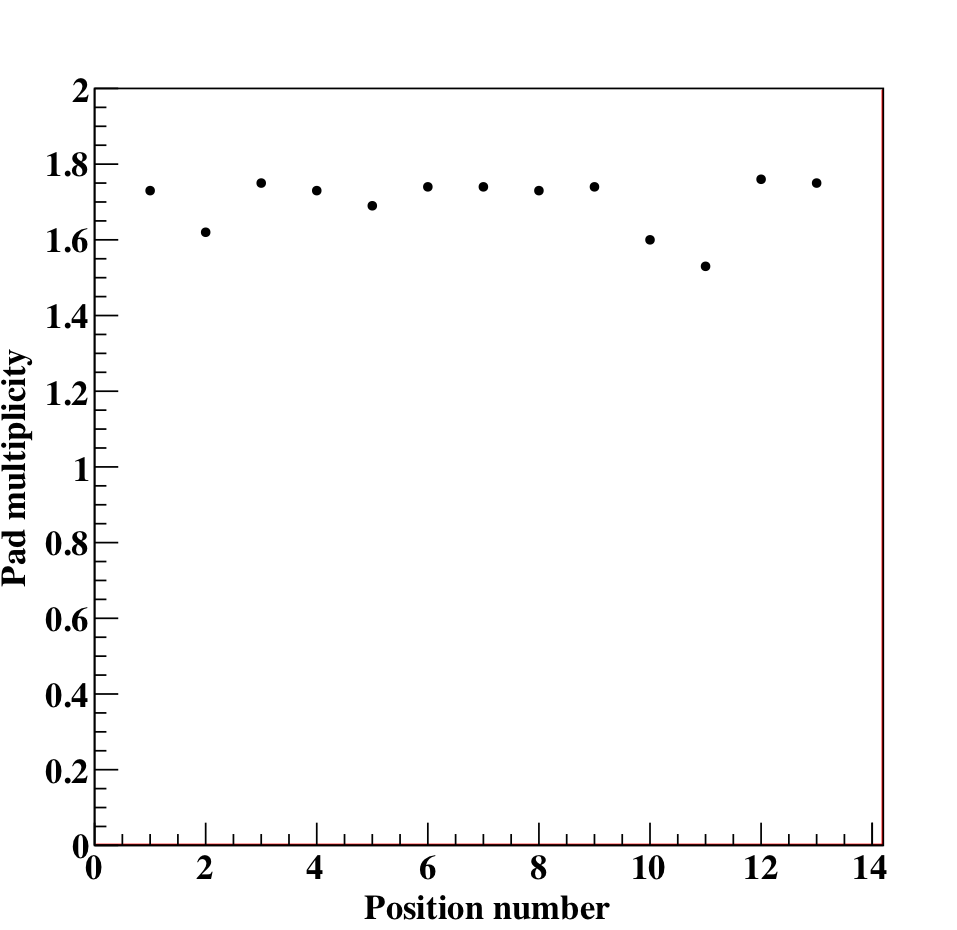
\includegraphics[width=0.9\textwidth]{images/Test1m2Multiplicity}}
\end{frame}
\begin{frame}{analog\_vs\_digital.eps}
  \centerline{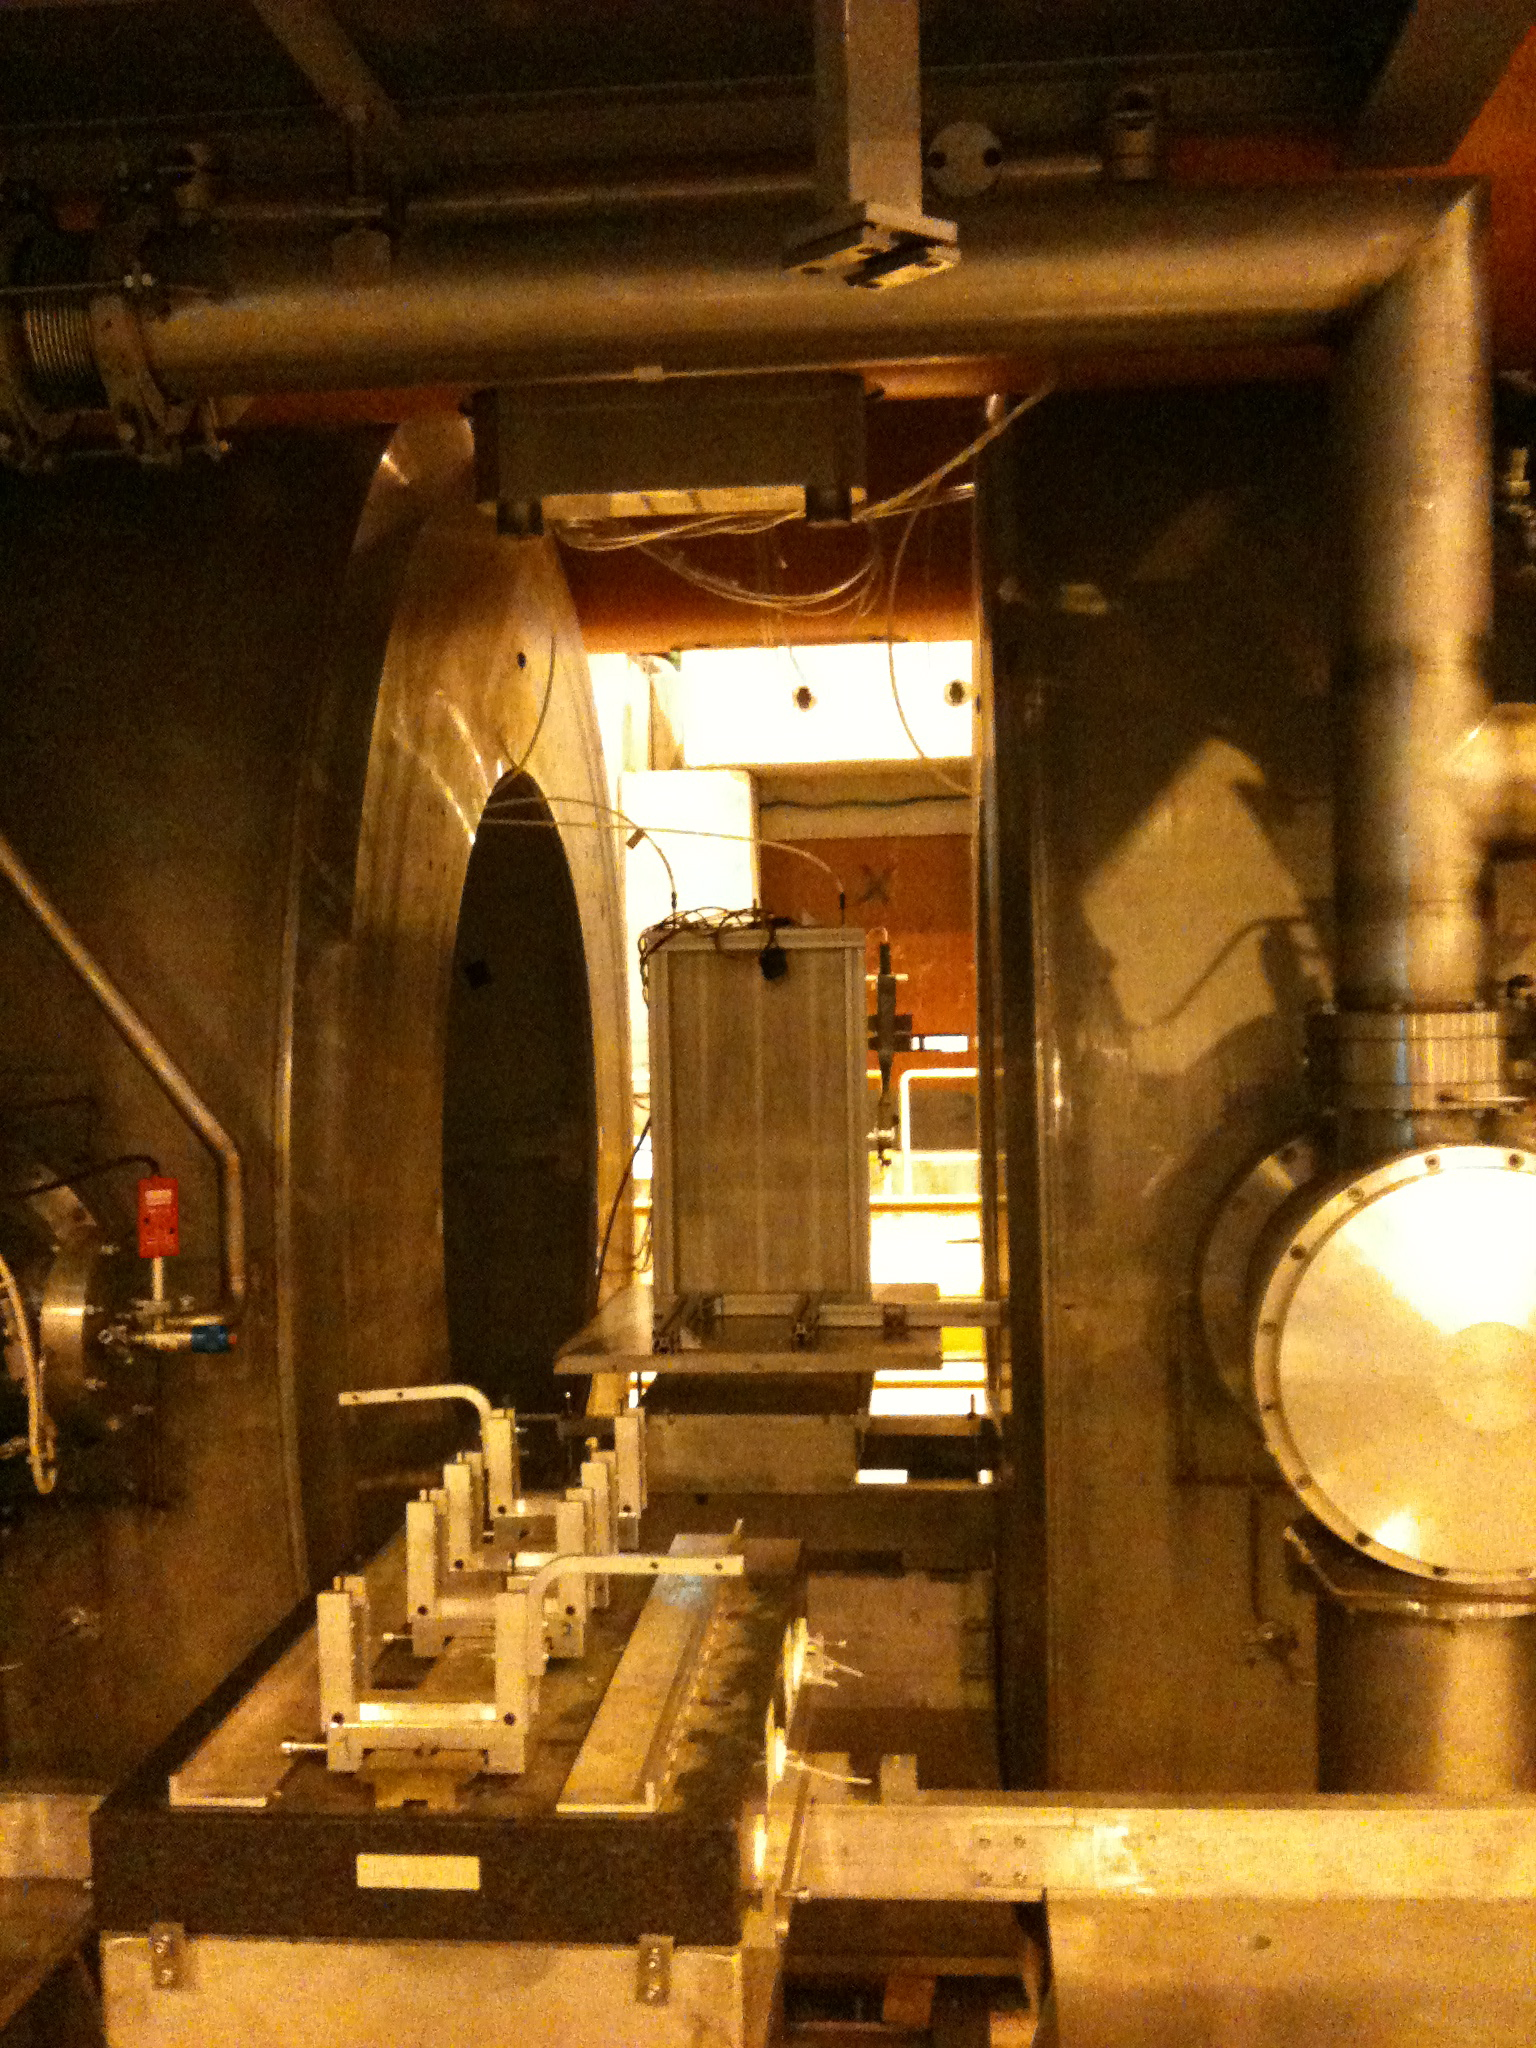
\includegraphics[width=0.9\textwidth]{images/PowerPulsingPhoto}}
\end{frame}
\begin{frame}{analog\_vs\_digital.eps}
  \centerline{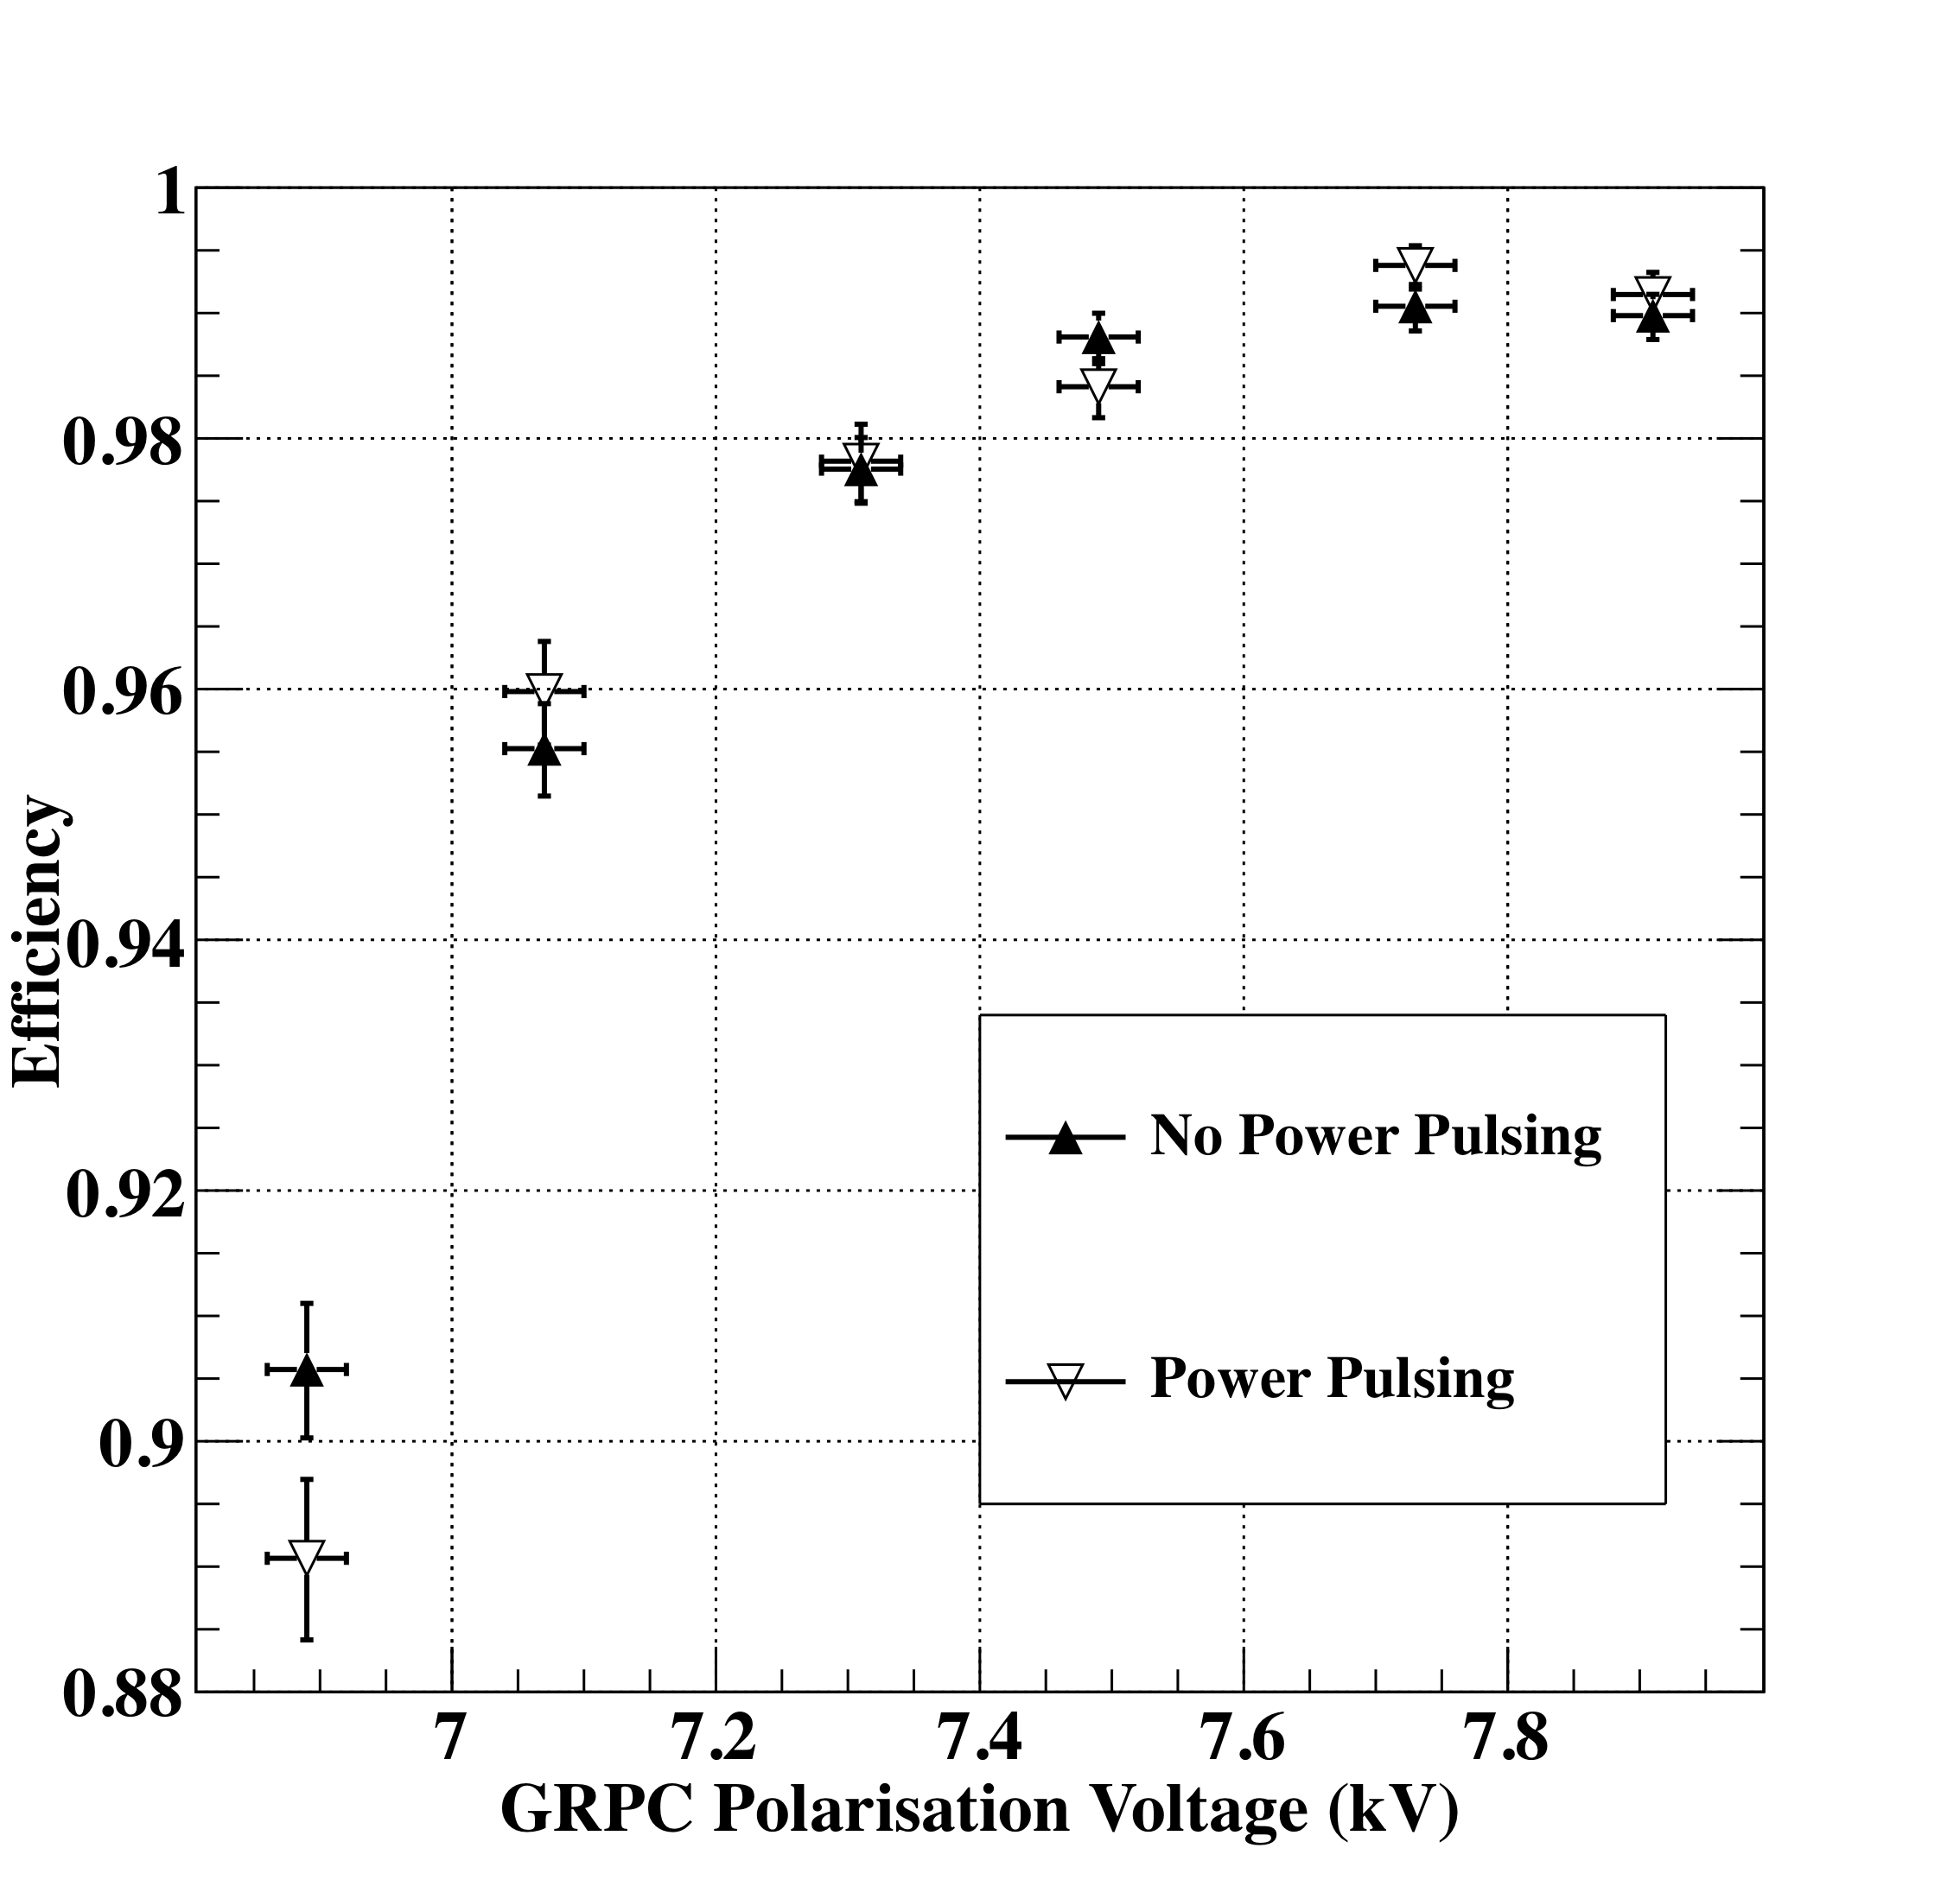
\includegraphics[width=0.9\textwidth]{images/PowerPulsingHvScan}}
\end{frame}

\begin{frame}{analog\_vs\_digital.eps}
  \centerline{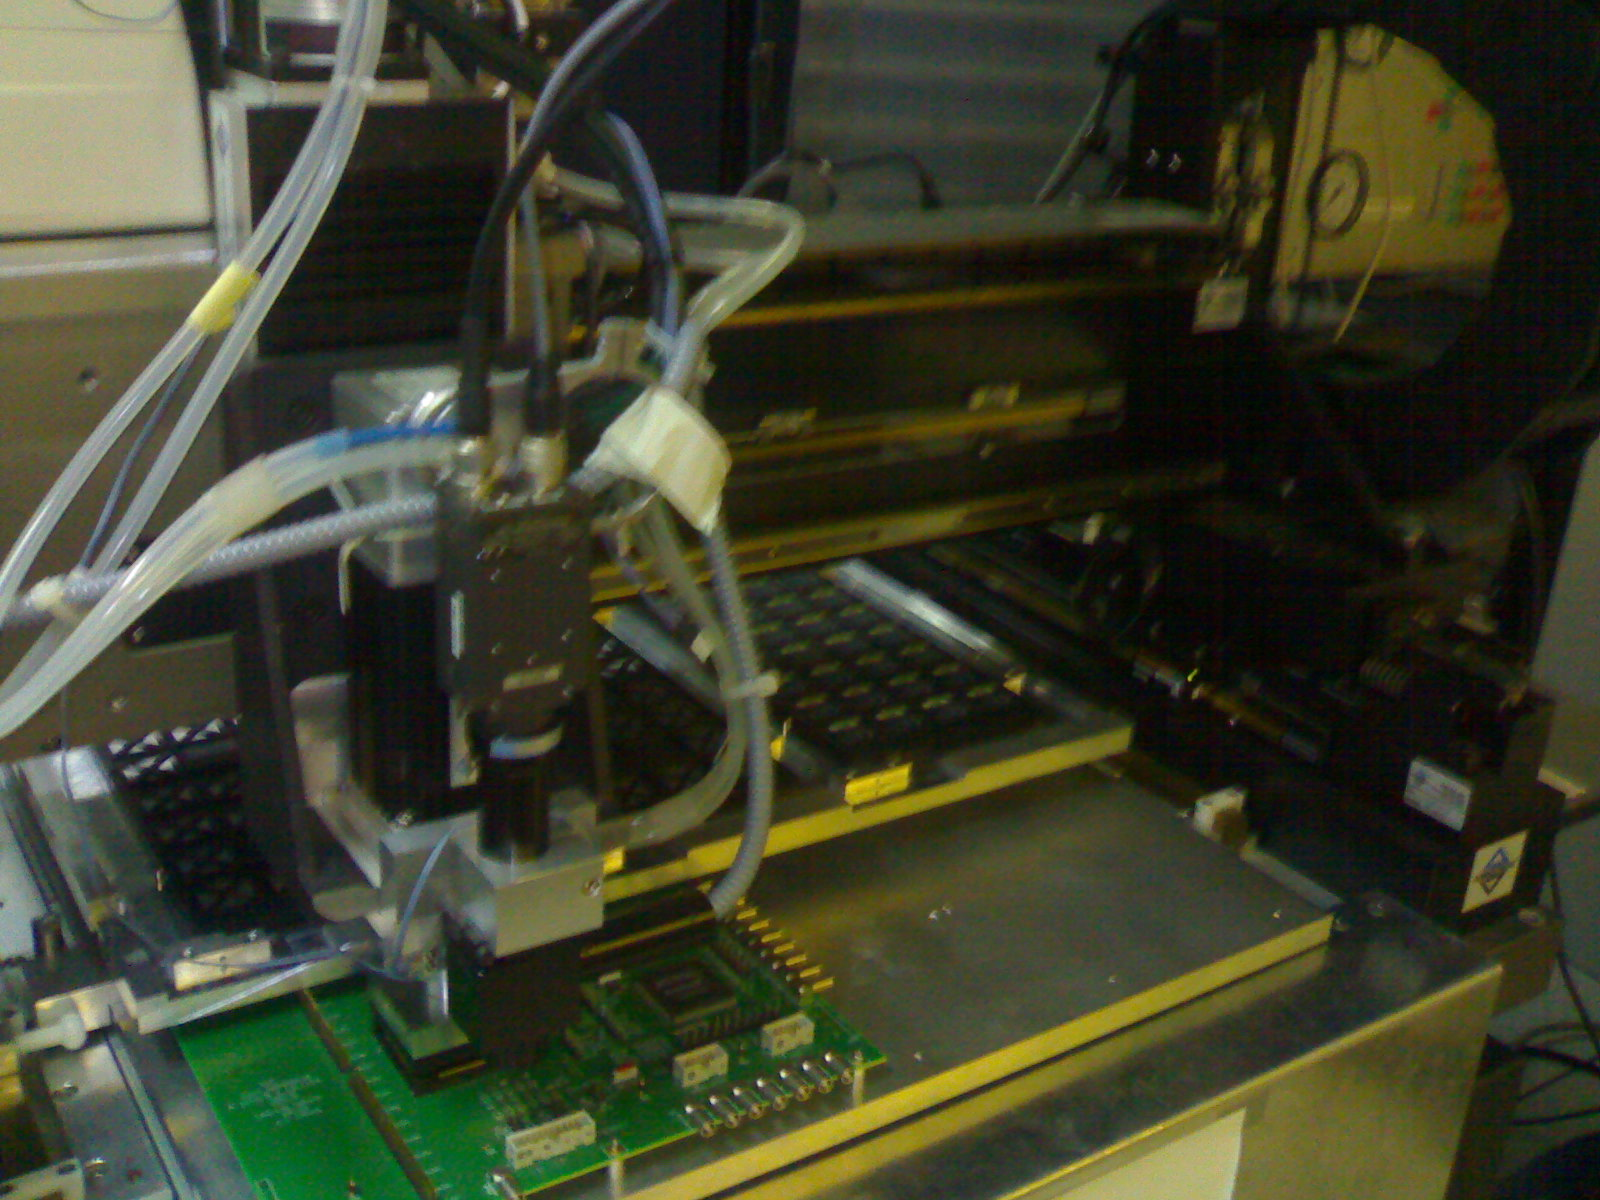
\includegraphics[width=0.9\textwidth]{images/ConstructionGantry}}
\end{frame}
\begin{frame}{analog\_vs\_digital.eps}
  \centerline{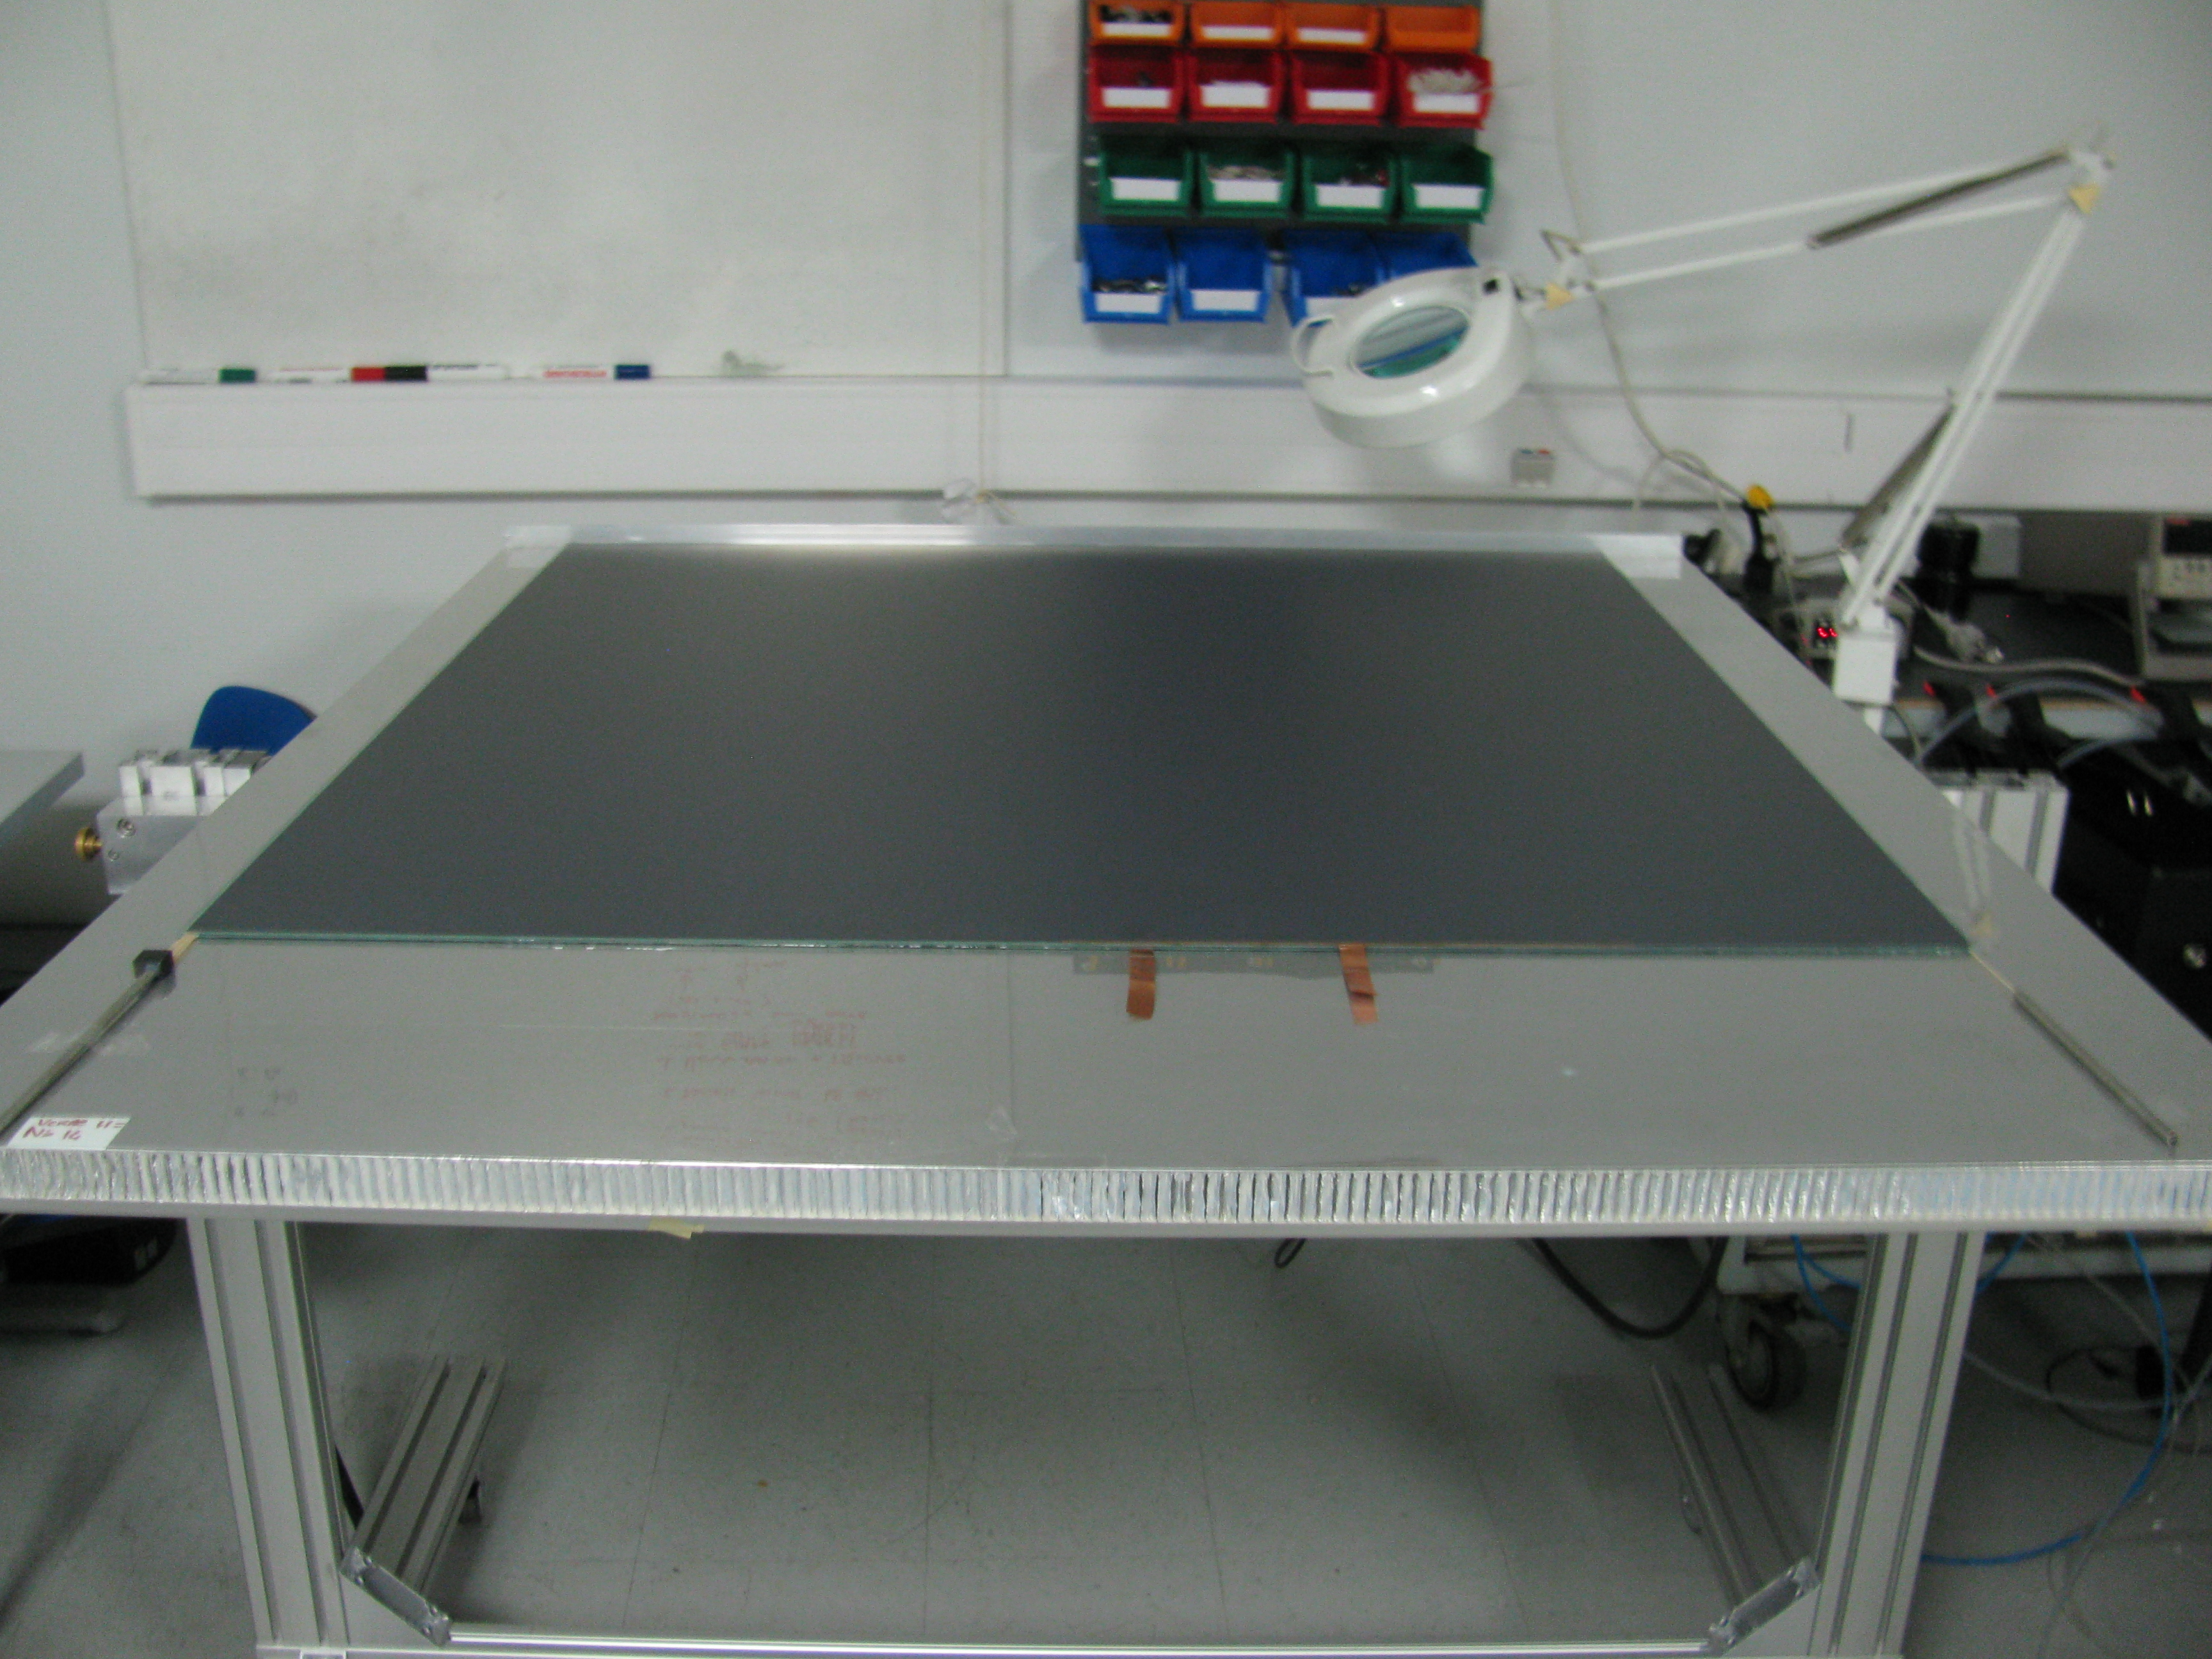
\includegraphics[width=0.9\textwidth]{images/ConstructionRPC}}
\end{frame}
\begin{frame}{analog\_vs\_digital.eps}
  \centerline{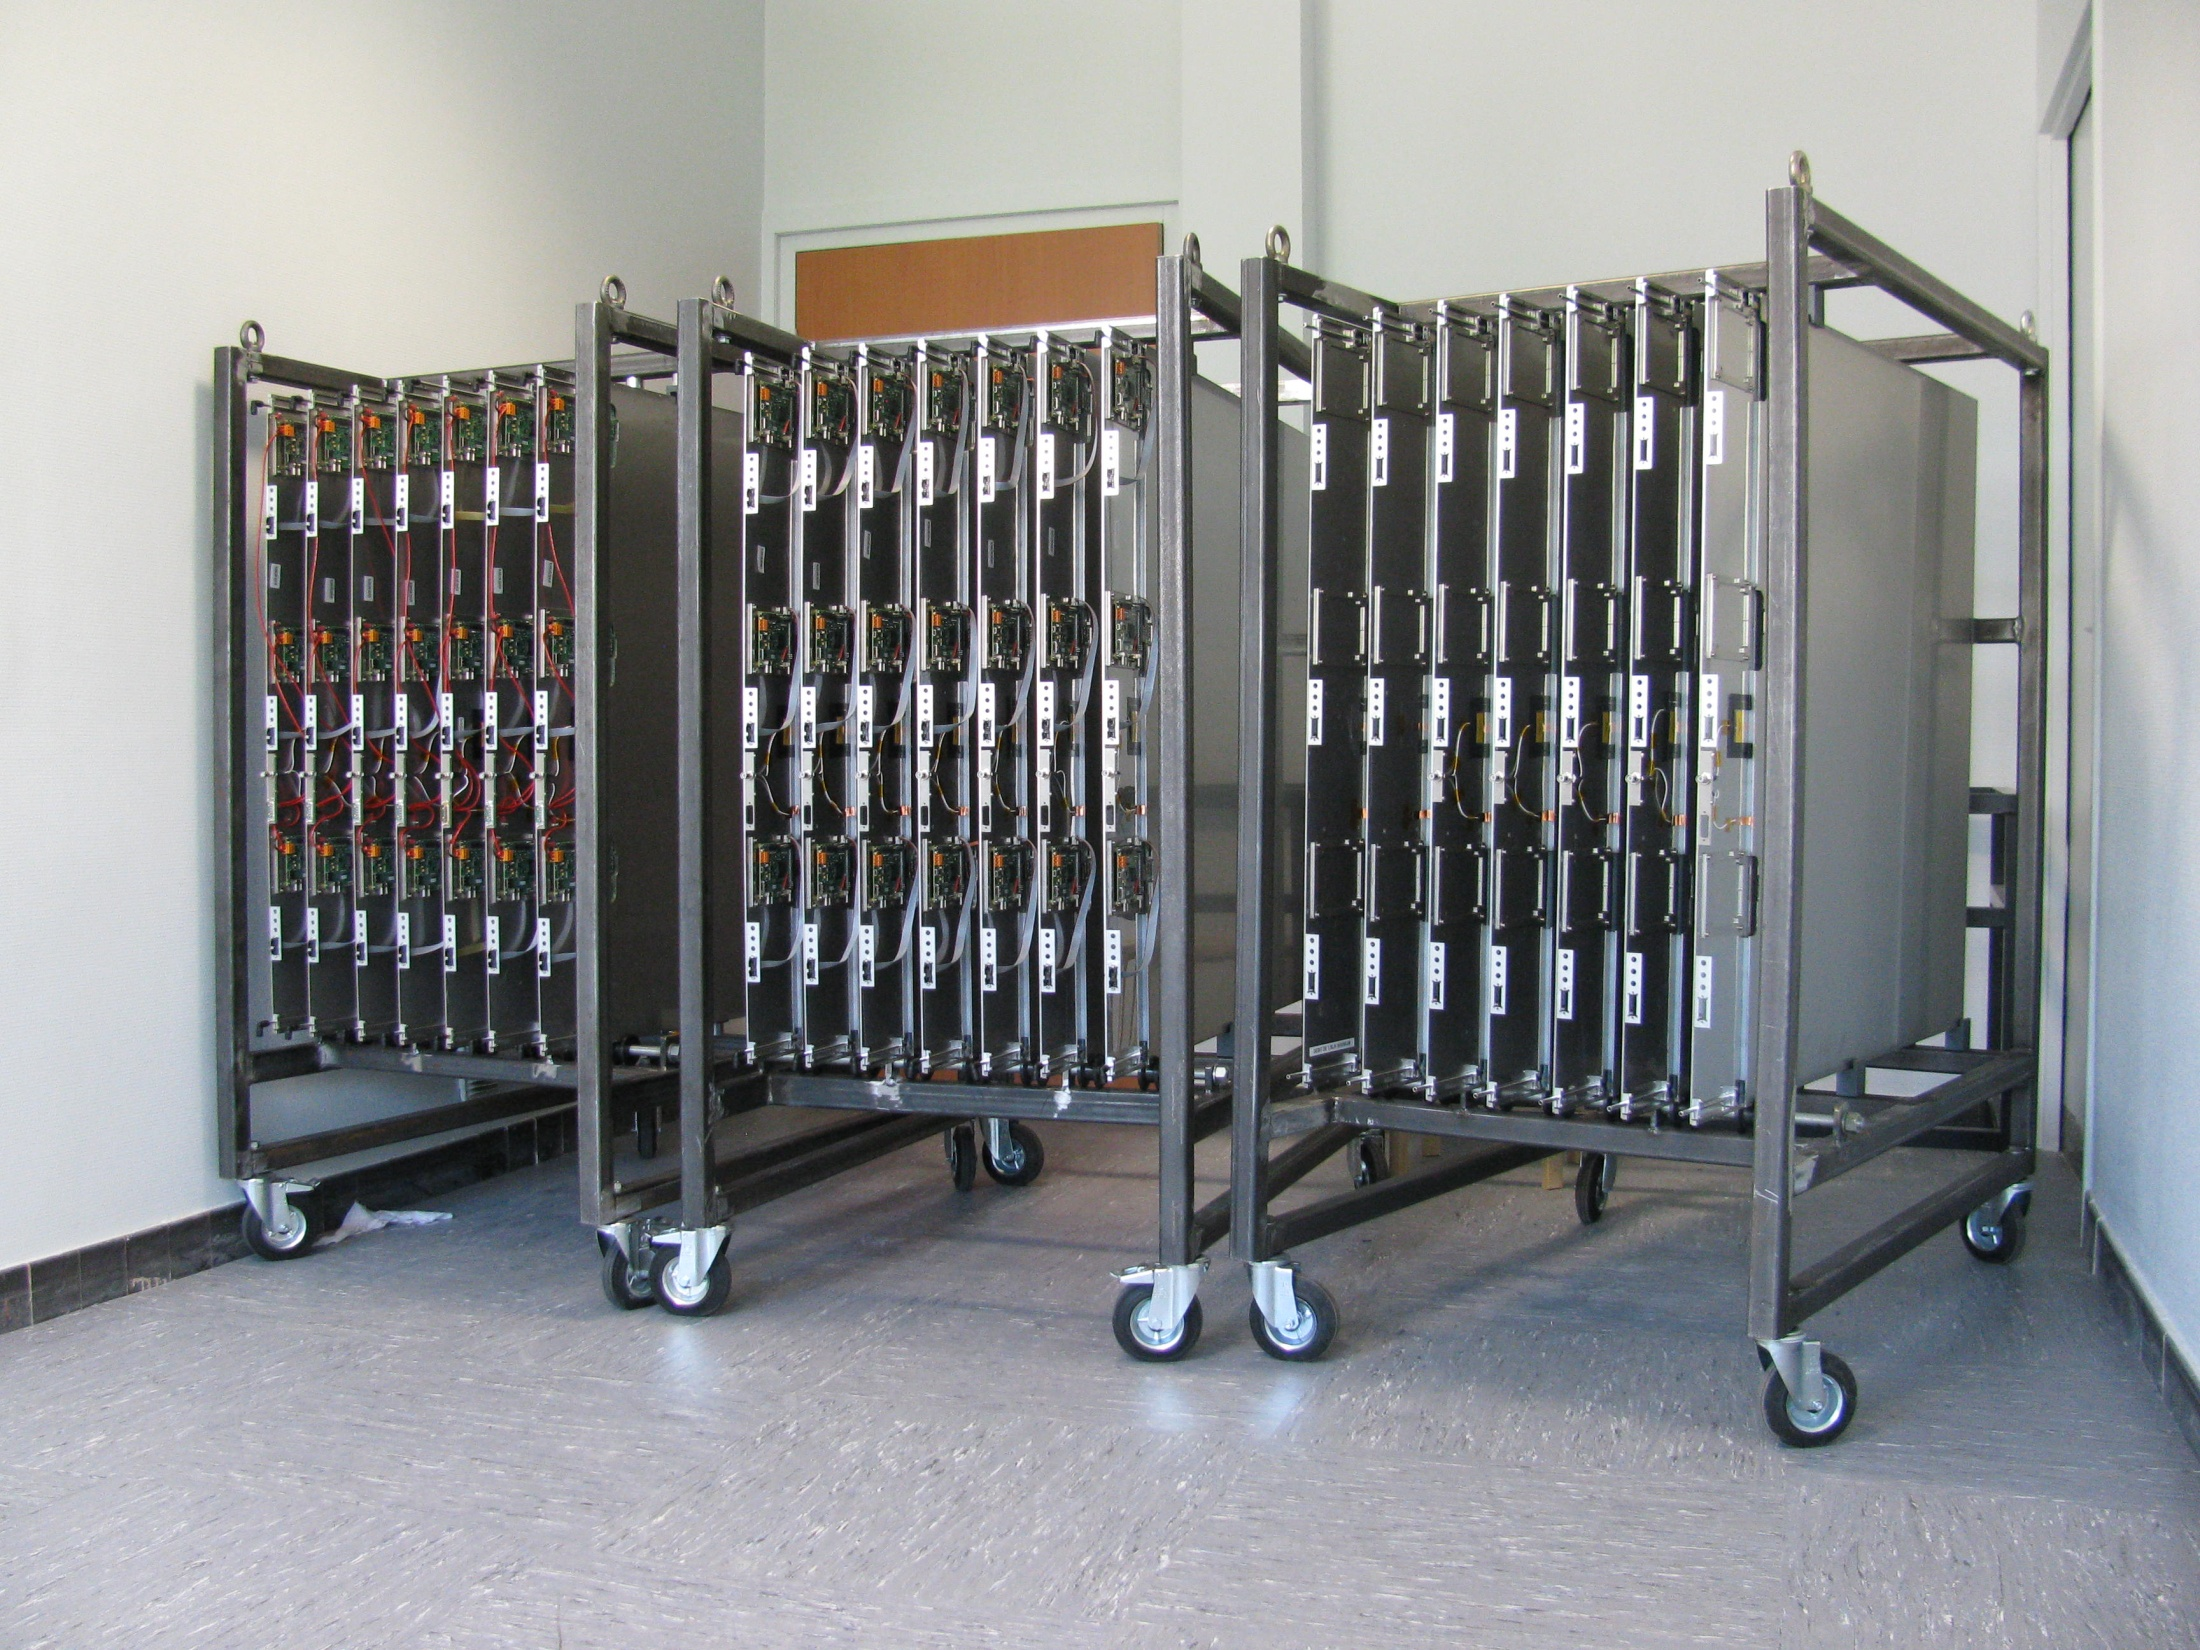
\includegraphics[width=0.9\textwidth]{images/ConstructionRack}}
\end{frame}
\begin{frame}{analog\_vs\_digital.eps}
  \centerline{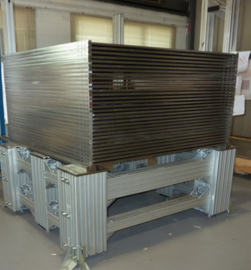
\includegraphics[width=0.9\textwidth]{images/ConstructionStructure}}
\end{frame}
\begin{frame}{analog\_vs\_digital.eps}
  \centerline{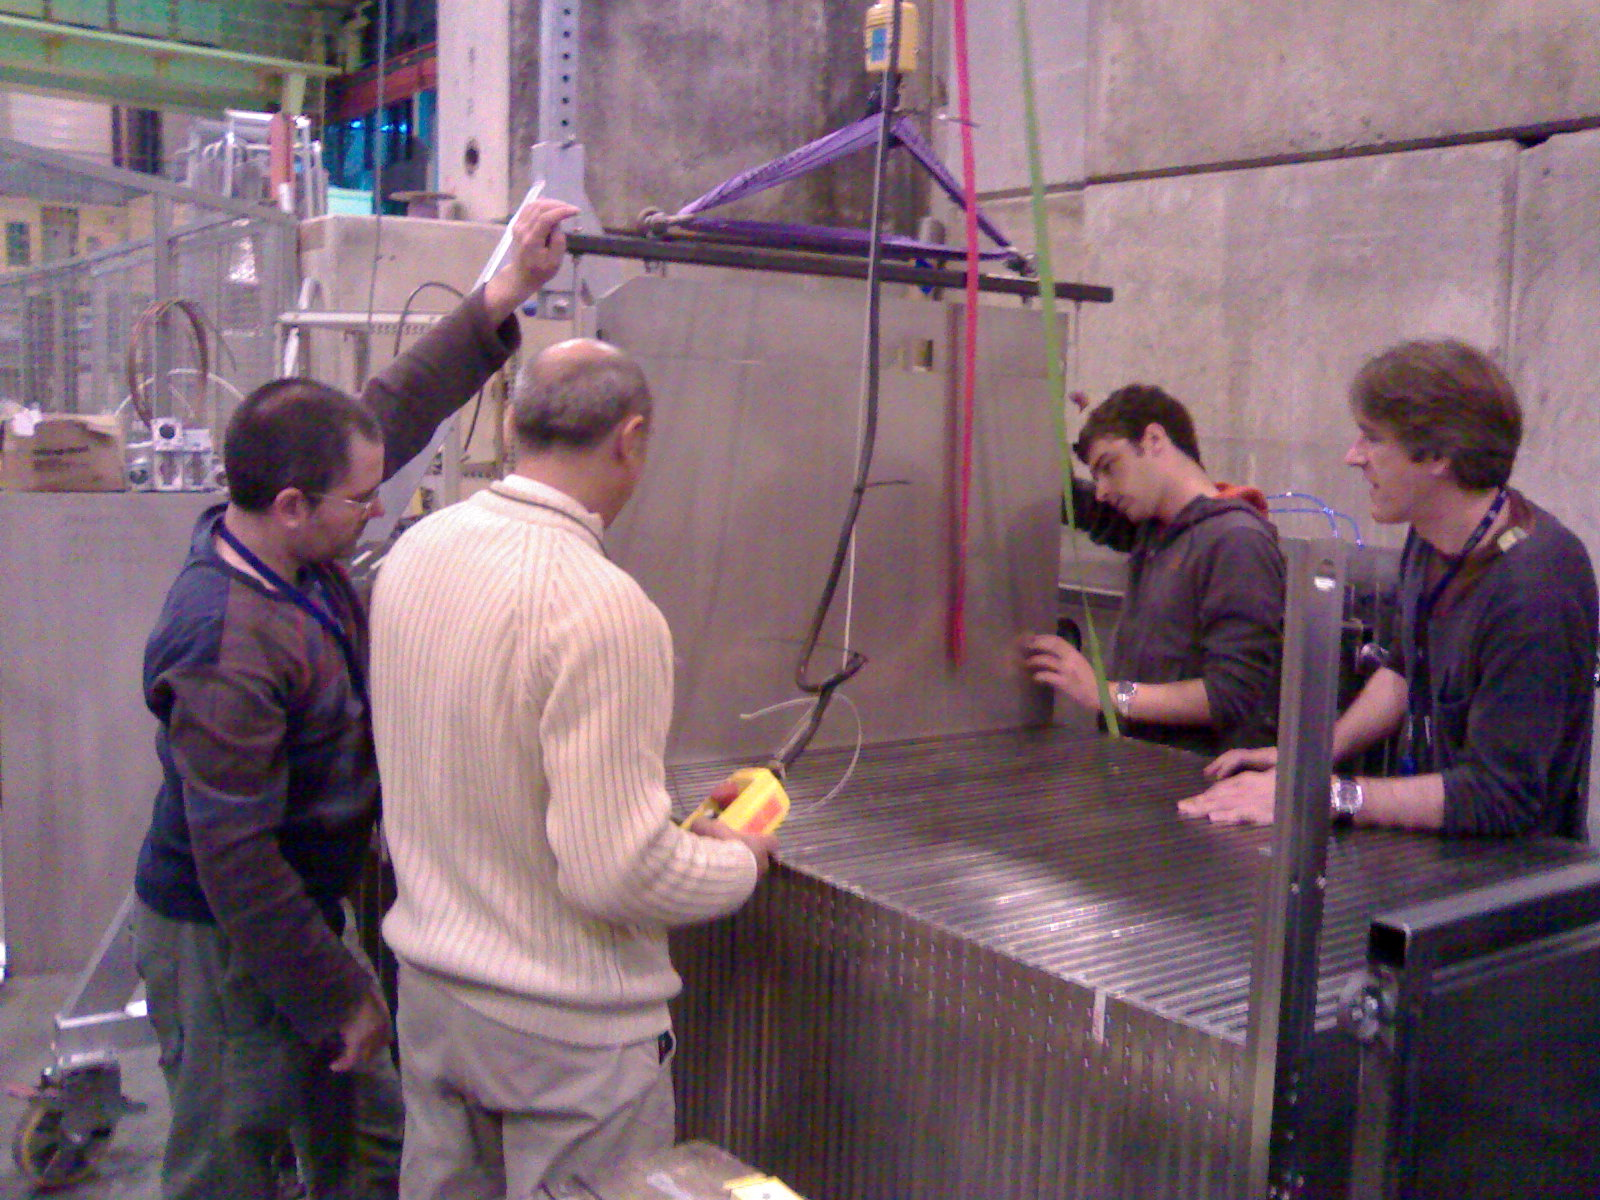
\includegraphics[width=0.9\textwidth]{images/ConstructionInsertion}}
\end{frame}


\begin{frame}{analog\_vs\_digital.eps}
  \centerline{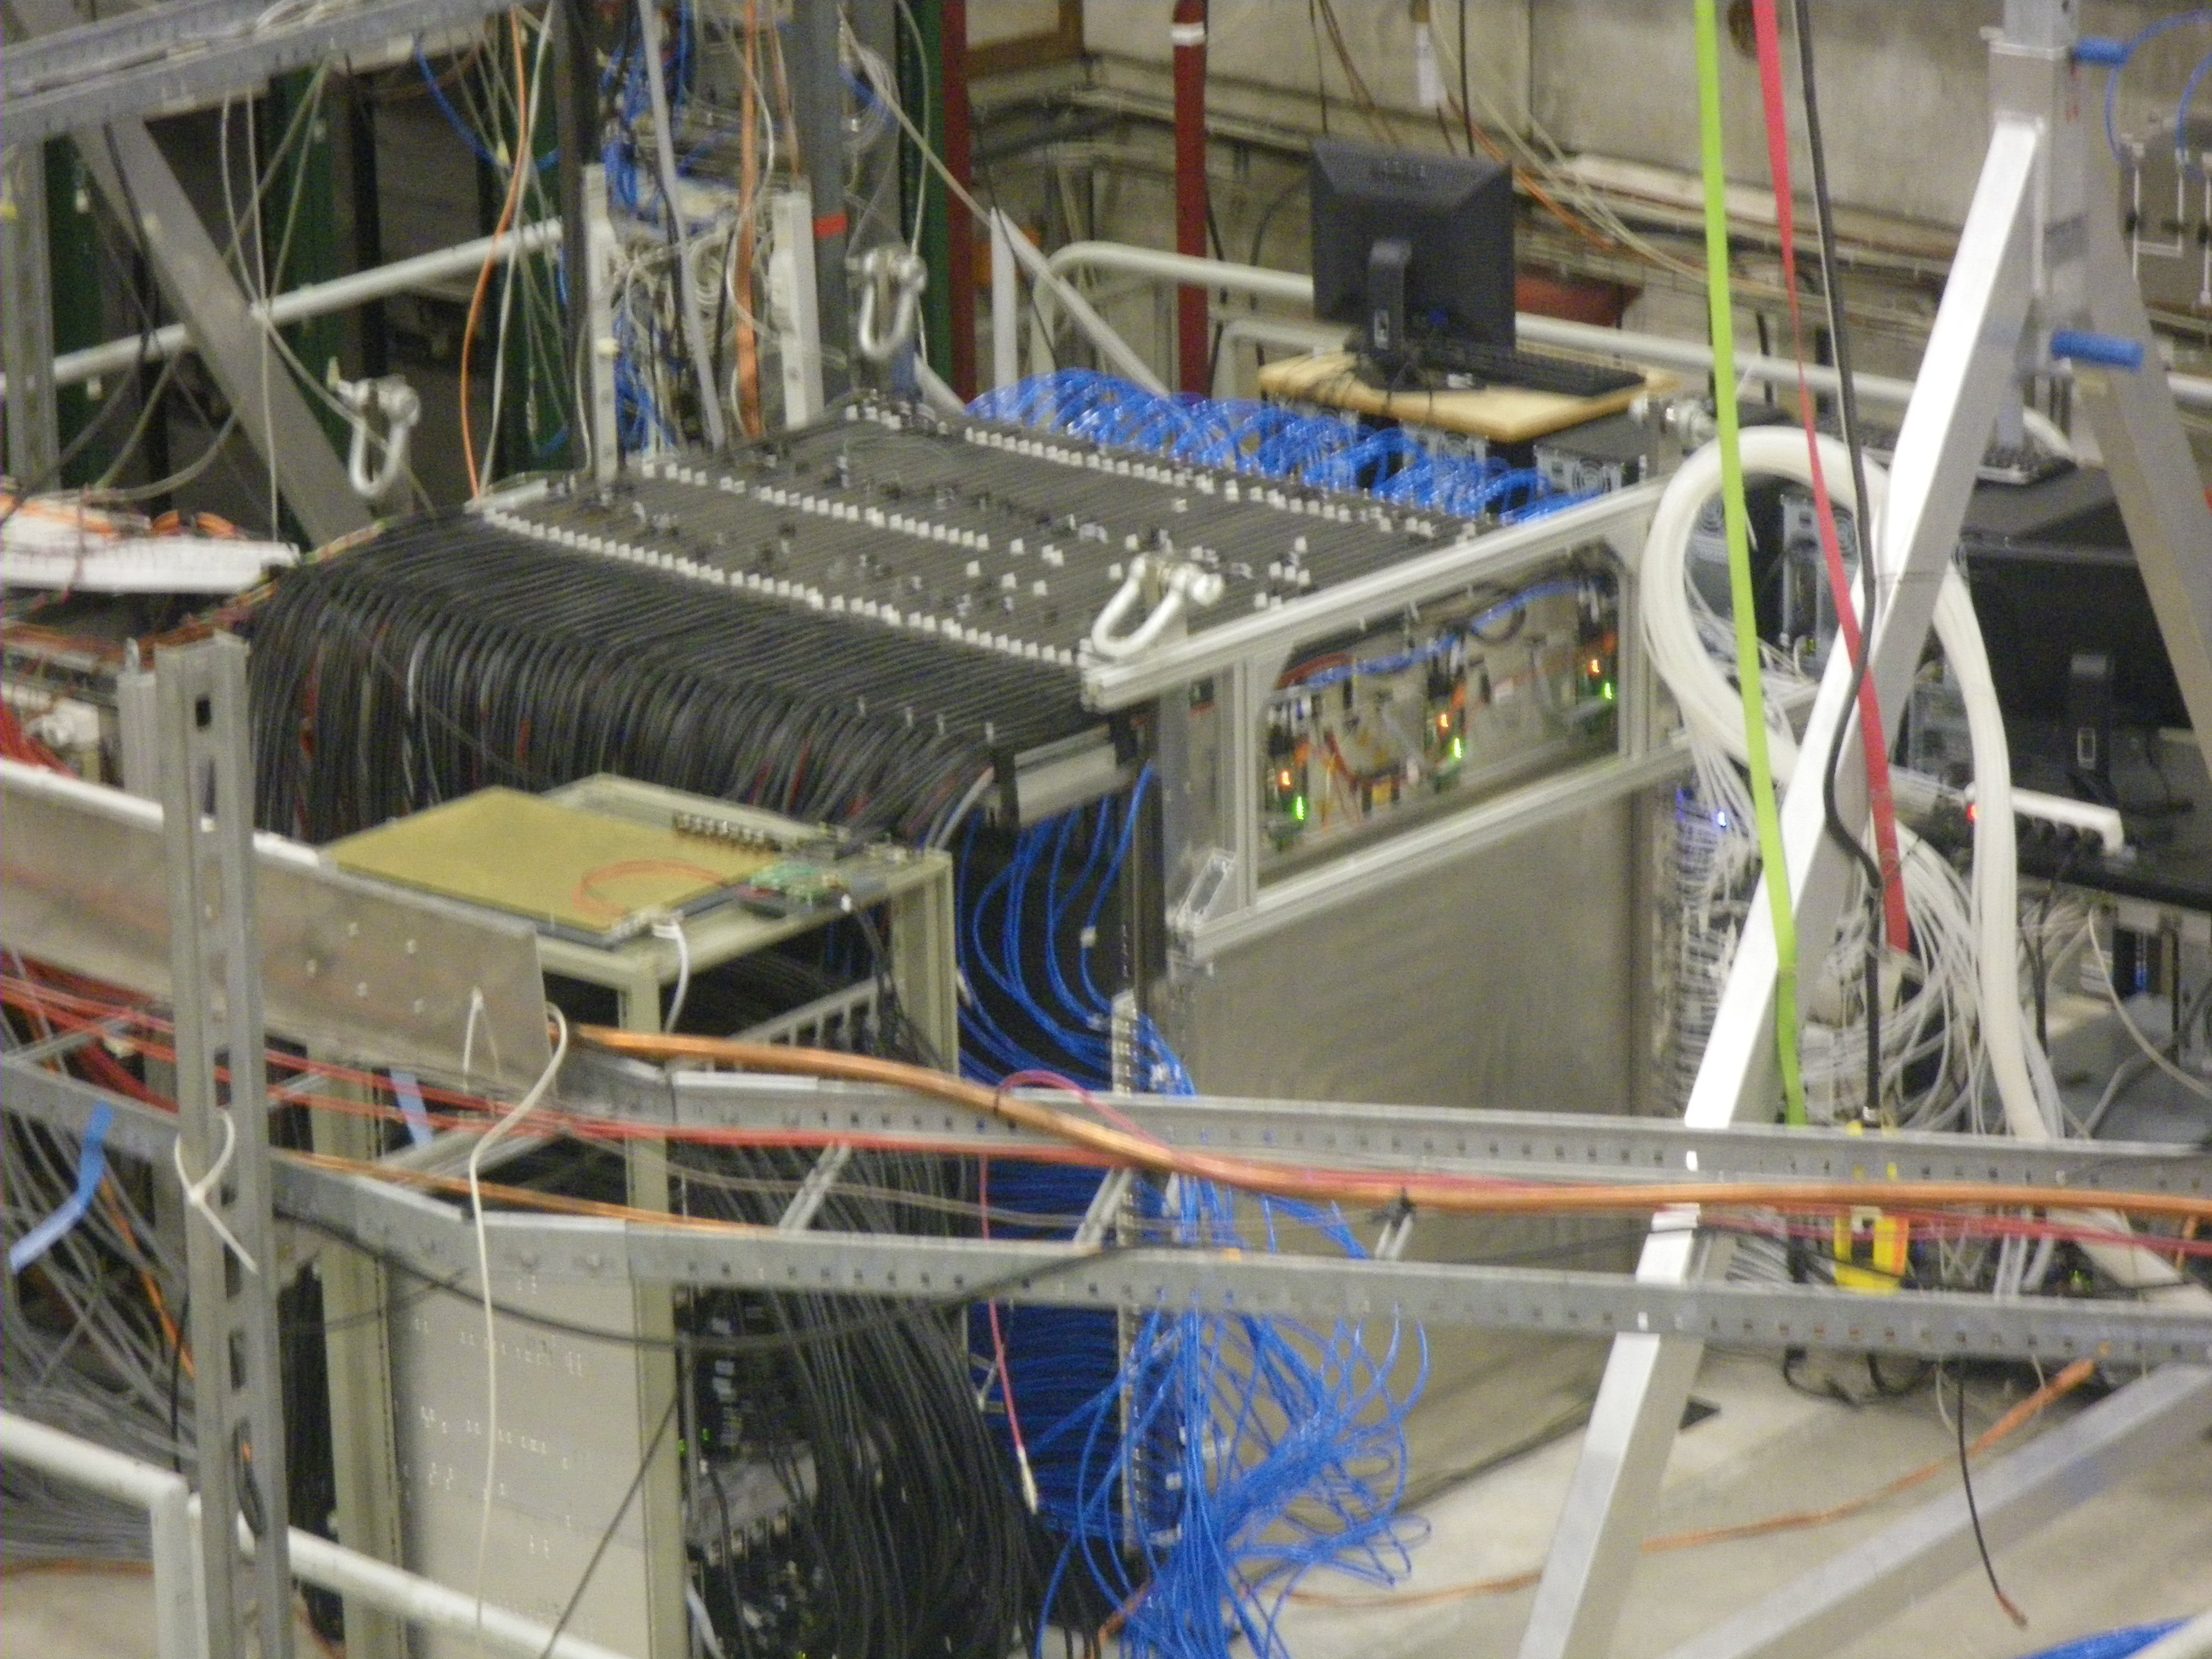
\includegraphics[width=0.9\textwidth]{images/1m3Photo}}
\end{frame}
\begin{frame}{analog\_vs\_digital.eps}
  \centerline{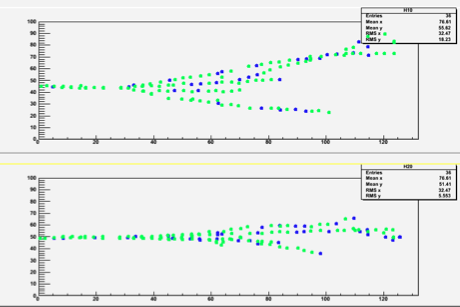
\includegraphics[width=0.9\textwidth]{images/10GevPion}}
\end{frame}
\begin{frame}{analog\_vs\_digital.eps}
  \centerline{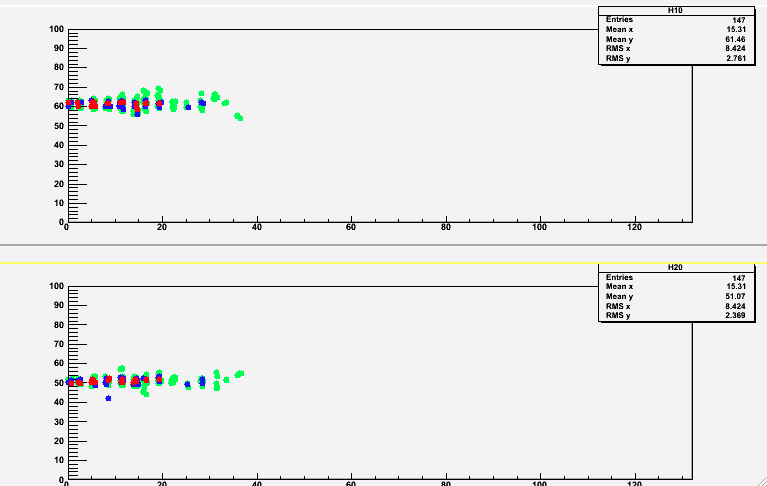
\includegraphics[width=0.9\textwidth]{images/10GevElectron}}
\end{frame}
\begin{frame}{analog\_vs\_digital.eps}
  \centerline{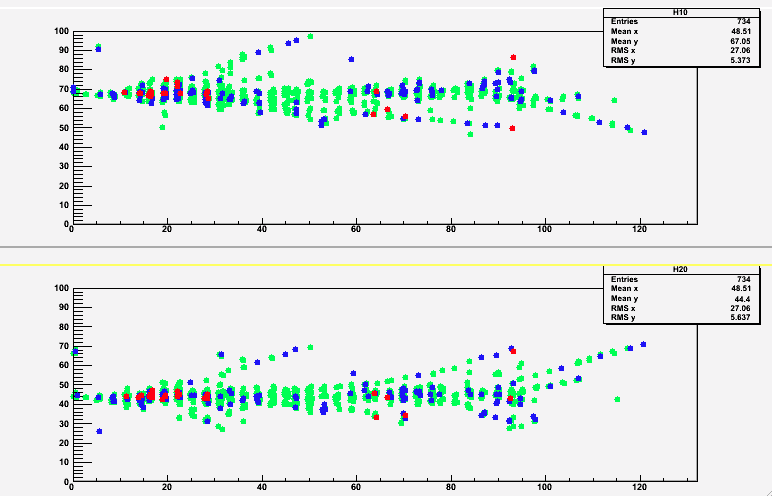
\includegraphics[width=0.9\textwidth]{images/50GevPion}}
\end{frame}
\begin{frame}{analog\_vs\_digital.eps}
  \centerline{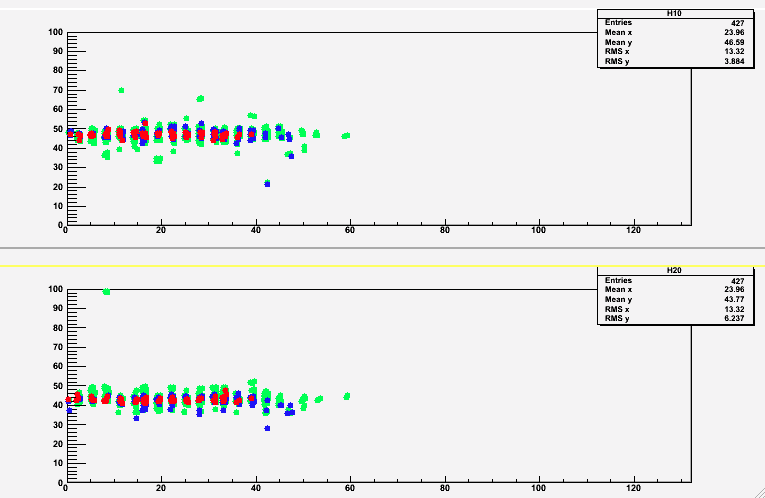
\includegraphics[width=0.9\textwidth]{images/50GevElectron}}
\end{frame}

\begin{frame}{analog\_vs\_digital.eps}
  \centerline{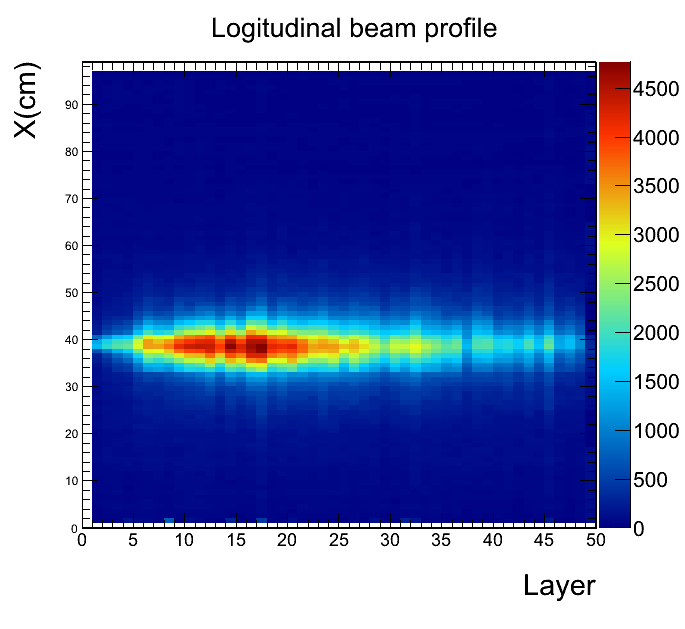
\includegraphics[width=0.9\textwidth]{images/Beam2012Longitudinal}}
\end{frame}
\begin{frame}{analog\_vs\_digital.eps}
  \centerline{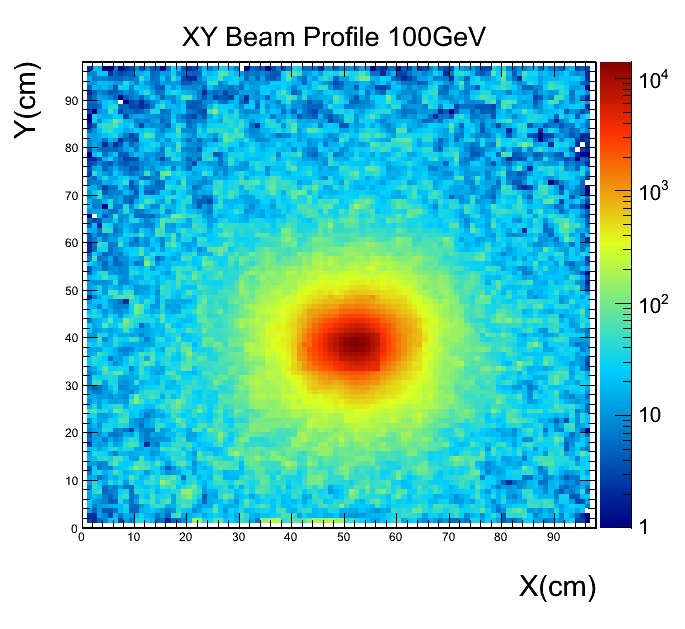
\includegraphics[width=0.9\textwidth]{images/Beam2012Transverse}}
\end{frame}
\begin{frame}{analog\_vs\_digital.eps}
  \centerline{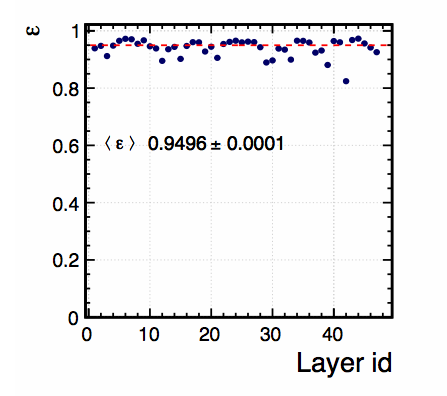
\includegraphics[width=0.9\textwidth]{images/Beam2012Efficiency}}
\end{frame}
\begin{frame}{analog\_vs\_digital.eps}
  \centerline{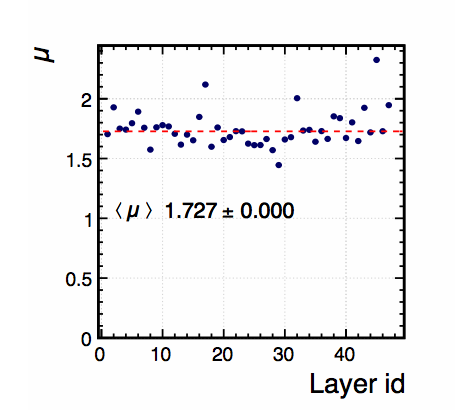
\includegraphics[width=0.9\textwidth]{images/Beam2012Multiplicity}}
\end{frame}
\begin{frame}{analog\_vs\_digital.eps}
  \centerline{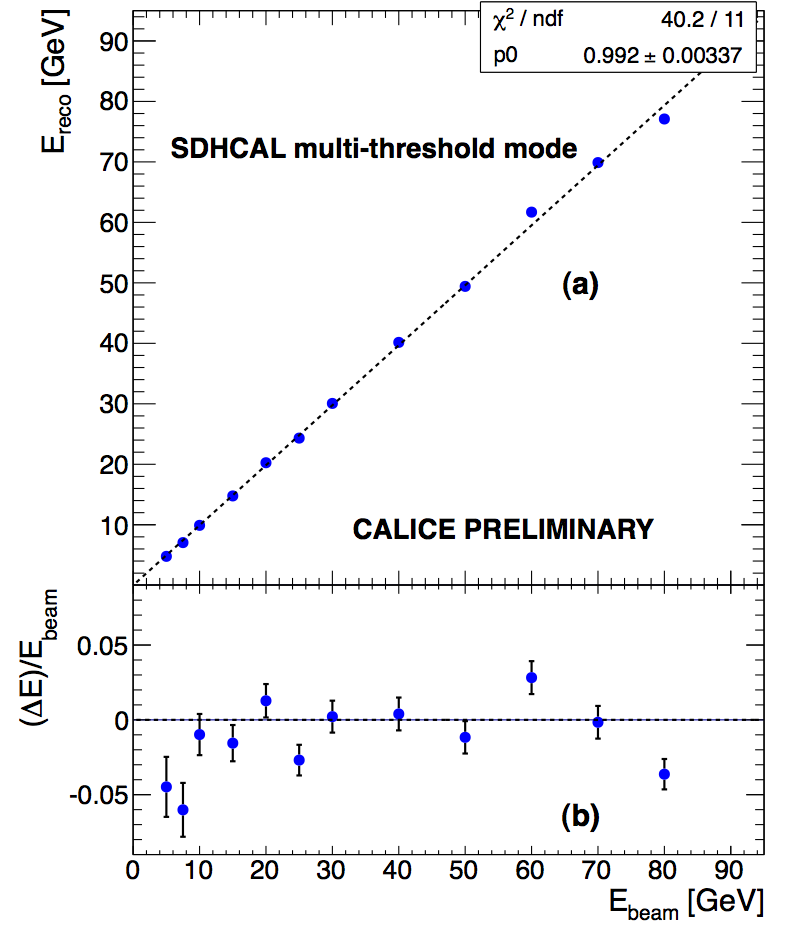
\includegraphics[width=0.9\textwidth]{images/Beam2012Linearity}}
\end{frame}

\begin{frame}{analog\_vs\_digital.eps}
  \centerline{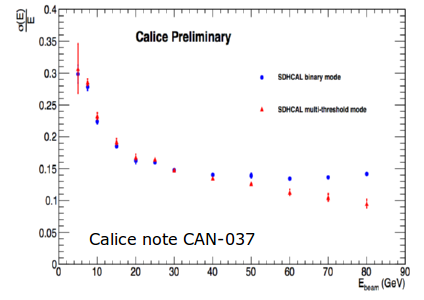
\includegraphics[width=0.9\textwidth]{images/Beam2012Resolution}}
\end{frame}
\begin{frame}{analog\_vs\_digital.eps}
  \centerline{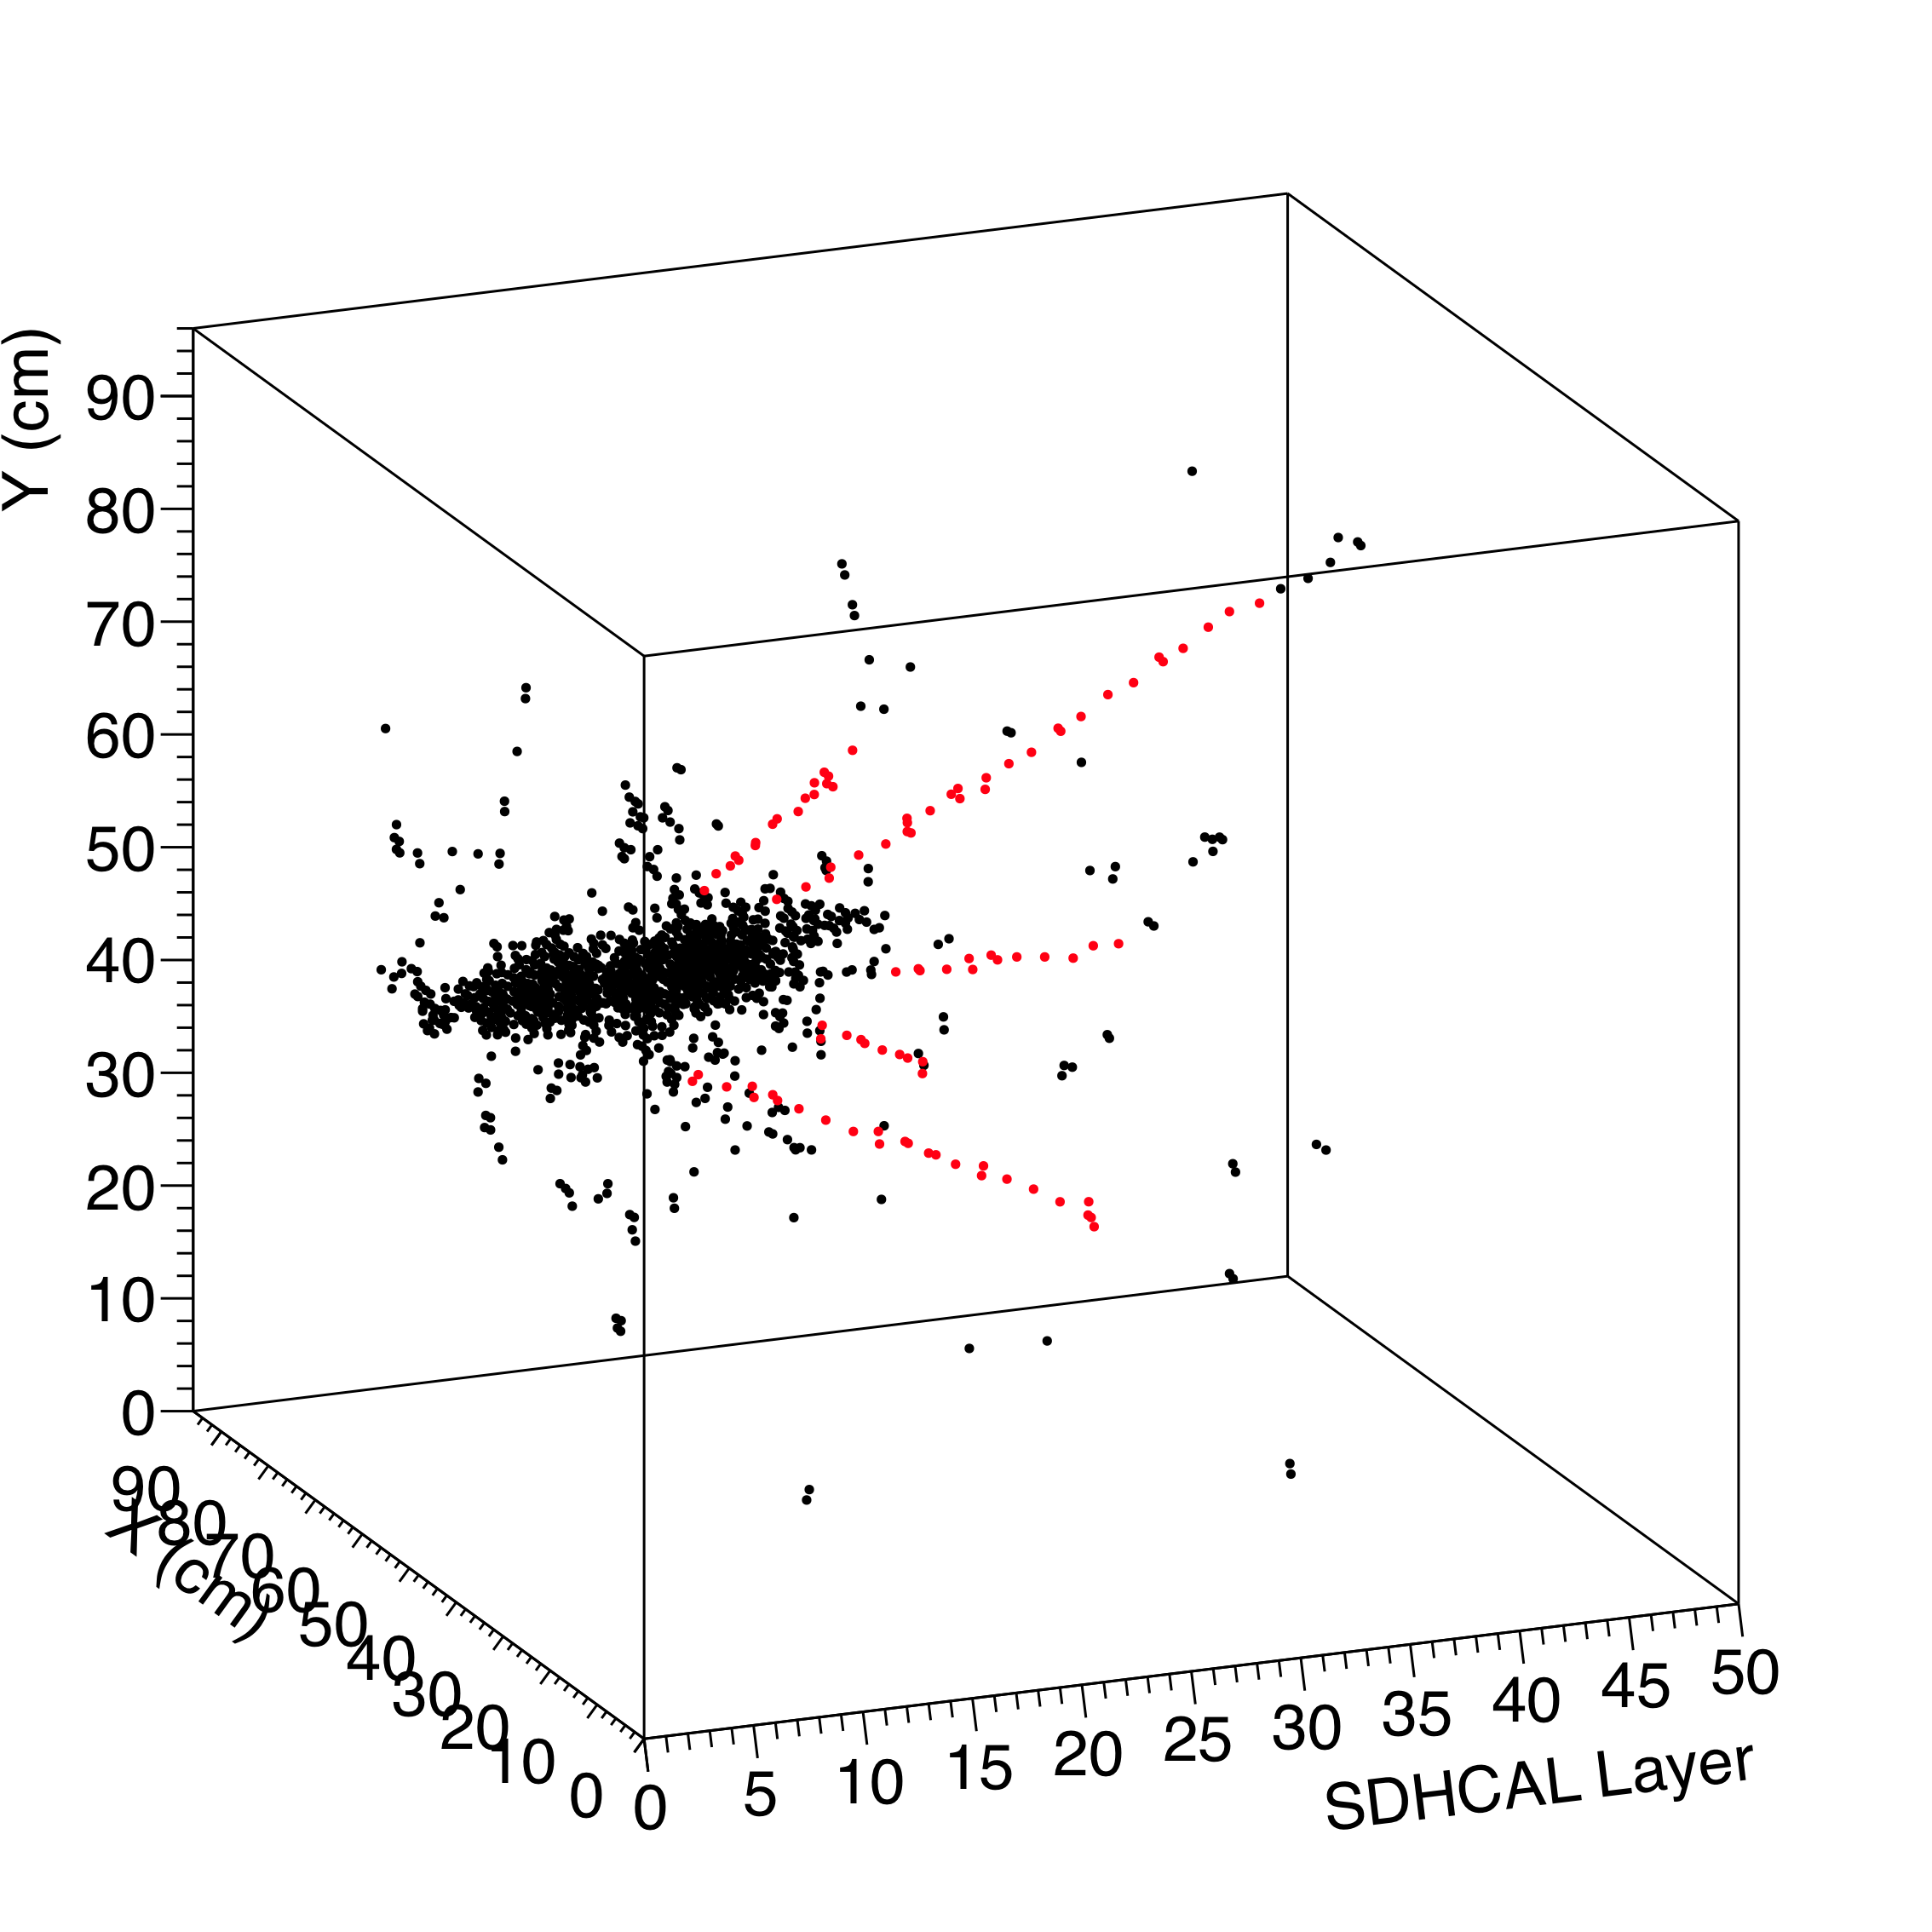
\includegraphics[width=0.9\textwidth]{images/Beam2012Hough}}
\end{frame}

\begin{frame}{analog\_vs\_digital.eps}
  \centerline{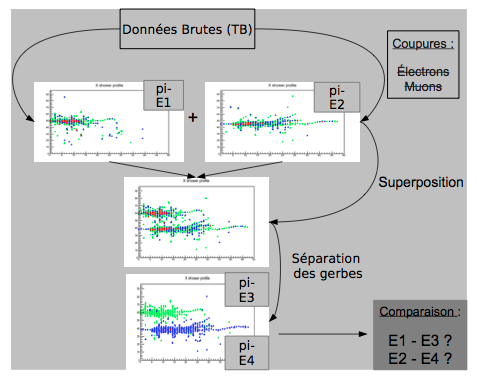
\includegraphics[width=0.9\textwidth]{images/Beam2012Arbor}}
\end{frame}



\section{Architecture}

\begin{frame}[shrink=5]{XDAQ}
  \begin{block}{Configuration}
    \begin{itemize}
    \item Executive : Web server dynamically loading application
    \item Each application appears as a servlet
    \item XML description of all executives and applications 
    \end{itemize}
  \end{block}
  \pause \begin{block}{Communication}
    \begin{itemize}
    \item Inside an Executive : Zero-copy
    \item Inside a PC: unix sockets
    \item Between PCs: tcp/ip sockets
    \end{itemize}
  \end{block}
  \pause 
  \begin{block}{User interface}
    \begin{itemize}
    \item Browser access of each application (CGI based)
    \item Web2 technology (AJAX, GWT)
    \item SOAP binding of the application
    \end{itemize}
  \end{block}
  
\end{frame}
\begin{frame}[fragile,shrink=60]
  \frametitle{XML configuration}

\begin{verbatim}
    <xc:Partition 
    

    <!-- Binary Network definition -->
    <i2o:protocol xmlns:i2o="http://xdaq.web.cern.ch/xdaq/xsd/2004/I2OConfiguration-30">
    <i2o:target class="DIFSupervisor" instance="0" tid="130"/>
    <i2o:target class="DIFSupervisor" instance="1" tid="131"/>
    <i2o:target class="BackupSaver" instance="0" tid="170"/>
    <i2o:target class="RUCollector"  instance="0" tid="37"/>
    <i2o:target class="LocalManager"  instance="0" tid="38"/>
    <i2o:target class="rubuilder::ru::Application"  instance="0" tid="41"/>
    <i2o:target class="rubuilder::bu::Application"  instance="0" tid="42"/>
    <i2o:target class="rubuilder::evm::Application"  instance="0" tid="43"/>
    <i2o:target class="rubuilder::fu::Application"  instance="0" tid="44"/>
    <i2o:target class="MarlinAnalyzer"  instance="0" tid="45"/>
    <i2o:target class="pt::atcp::PeerTransportATCP"  instance="0" tid="47"/>
    </i2o:protocol>

    <!-- One executive definition -->

    <xc:Context url="http://lyoac20:10000">
    <xc:Endpoint hostname="lyoac20" network="dhcalatcp" port="31805" protocol="atcp" service="i2o" />

    <!-- DIF supervisor #0-->
    <xc:Application class="DIFSupervisor" id="30" instance="0"  network="local">      <properties xmlns="urn:xdaq-application:DIFSupervisor" xsi:type="soapenc:Struct">
    <UseBackup xsi:type="xsd:boolean">false</UseBackup>
    <UseShm xsi:type="xsd:boolean">true</UseShm>	
    <UseCCC xsi:type="xsd:boolean">true</UseCCC>
    <UseDB xsi:type="xsd:boolean">false</UseDB>	
    <ASICType xsi:type="xsd:integer">2</ASICType>
    <ASICHeaders xsi:type="xsd:string">1 2 3 4 5 6 7 8 9 10 11 12 13 14 15 16 17 18 19 20 21 22 23 24 25 26 27 28 29 30 31 32 33 34 35 36 37 38 39 40 41 42 43 44 45 46 47 48</ASICHeaders>
    <DIF_Identifier xsi:type="xsd:string">FT101002</DIF_Identifier>
    </properties>
    </xc:Application>
    ...
    <!-- Library to load -->
    <xc:Module>/opt/xdaq/lib/libptatcp.so</xc:Module>
    <xc:Module>/usr/local/lib/libftd2xx.so</xc:Module>
    <xc:Module>/data/online/opt/dhcal/lib/libRUCollector.so</xc:Module>
    <xc:Module>/data/online/opt/dhcal/lib/libDIFSupervisor.so</xc:Module>
    ...
\end{verbatim}

\end{frame}

\begin{frame}[shrink=5]{The CMS Event Builder}

  See {\tiny http://cms-ru-builder.web.cern.ch/cms-ru-builder/RUBUILDER\_G\_V1\_6\_0.doc}



  {\sl Aysnchronous collection of data source corresponding to the same trigger.}

  \bigskip
  \begin{columns}
    \begin{column}{0.5\textwidth}
      \begin{itemize}
      \item {\small One trigger is seen}
      \item {\small Each R{\sl eadout}U{\sl nit}I{\sl nput} collects its fragments and pushes it to the RU}
      \item {\small The T{\sl rigger}A{\sl ccepter} sends trigger data to the EV{\sl ent}M{\sl anager} }
      \item {\small The {\bf EVM} sends an event Id to the {\bf B}{\sl uilder}{\bf U}{\sl nit} that will request its first buffer to each {\bf RU} and build the event}
      \item {\small The event is sent to the registered {\bf F}{\sl ilter}{\bf U}{\sl nit} that can make data coherence checks, analysis and data storage}
      \end{itemize}
    \end{column}

    \begin{column}{0.65\textwidth}
      \centerline{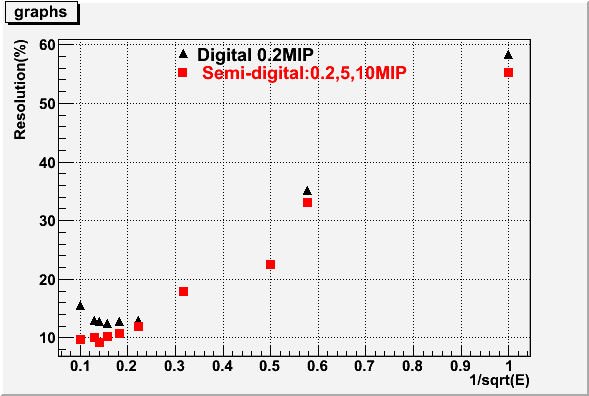
\includegraphics[width=0.9\textwidth]{images/DigitalSemiDigital}}
    \end{column}
  \end{columns}
\end{frame}

\begin{frame}{The DHCAL case}
  \centerline{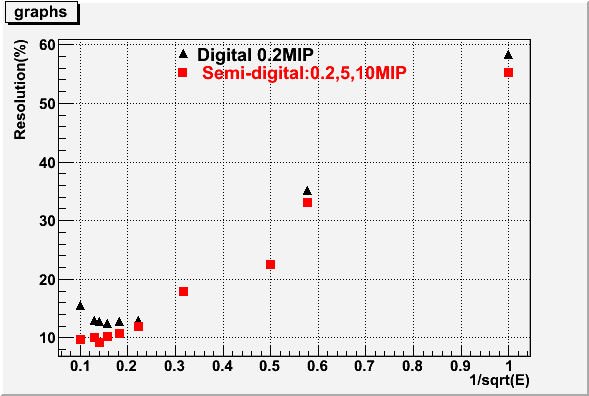
\includegraphics[width=0.9\textwidth]{images/DigitalSemiDigital}}
\end{frame}

\begin{frame}{Including the analysis}

  \begin{block}{ To do}
    \begin{enumerate}
    \item Data coherency and event building
    \item LCIO storage
    \item Monitoring
    \end{enumerate}
  \end{block}
  \pause 
  \begin{block}{ Implementation}
    \begin{itemize}
    \item Separe FU (CMS) application to DHCAL ones: Event forwarded to an {\sl LCIOAnalyzer } or {\sl MarlinAnalyzer}
    \item Custom LCIO Event building and storage (DHCalAnalysis library)
    \item Monitoring using an online interface to MARLIN (MarlinAnalyzer)
    \end{itemize}
  \end{block}

\end{frame}

\section{Data collection}

\begin{frame}{Using share memories}


  \begin{columns}
    \begin{column}{0.5\textwidth}
      {\bf class RUShare } 
      \begin{itemize}
      \item <1-> Creation of a named Share memory (server) or attachment to it
      \item <1-> Mapped to 100 Slots of 512kBytes
      \item <1-> Slot status FREE,READY,LOCK
      \item <2->Server (data source) looks for FREE slot, lock it and write data and mark it READY
      \item <2->Client (consumer ) look for READY slot , lock it, read data and mark it FREE
      \end{itemize}
    \end{column}
    \begin{column}{0.65\textwidth}
      \only<2->
          {
            \centerline{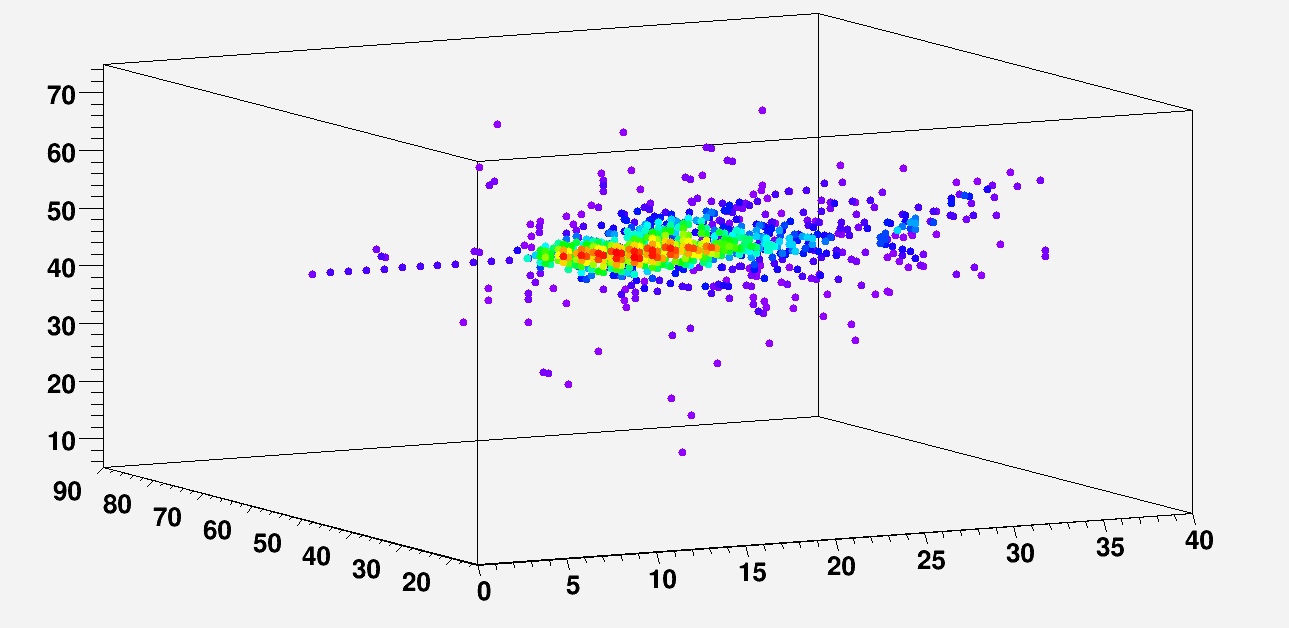
\includegraphics[width=0.9\textwidth]{images/ShowerExample}}
          }
    \end{column}
  \end{columns}
\end{frame}

\begin{frame}{Using share memories}
  \begin{columns}
    \begin{column}{0.5\textwidth}
      \begin{block}{Servers}
        Each {\sl DIFSupervisor} is a data source: it creates and fills one share memory, one trigger to one slot
      \end{block}
      \pause 
      \begin{block}{Client}
        The {\sl RUCollector} is the unique client of a set of DIFSupervisor
        \begin{itemize}
        \item it loops on the 100 slots and looks for READY slots on ALL share memories
        \item it copies data from the same slot(same trigger) and FREE the slots
        \item it pushes the collected data to the Event Builder 
        \end{itemize}
      \end{block}
    \end{column}
    \begin{column}{0.5\textwidth}
      \centerline{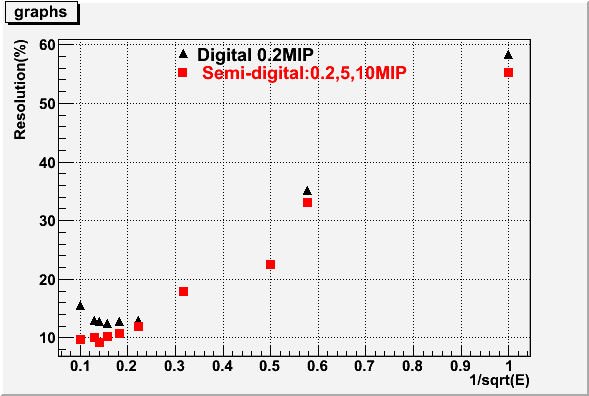
\includegraphics[width=0.9\textwidth]{images/DigitalSemiDigital}}
    \end{column}
  \end{columns}


\end{frame}

\begin{frame}{Several PC's}

  \begin{columns}
    \begin{column}{0.5\textwidth}

      \begin{block}{Constraint}
        \begin{itemize}
        \item DIFSupervisor's should run on the PC where the DIF are connected 
        \item one RUCollector per PC reading DIF
        \end{itemize}
      \end{block}
      \pause
      \begin{block}{Distributed Event building and analysis}
        Any number of BU/FU can be added on the same or on other PCs

        The whole configuration is described in an XML file and the reorganisation of the applications is easy ({\sl to move analysis to a new PC for example})
      \end{block}
    \end{column}
    \begin{column}{0.5\textwidth}
      \centerline{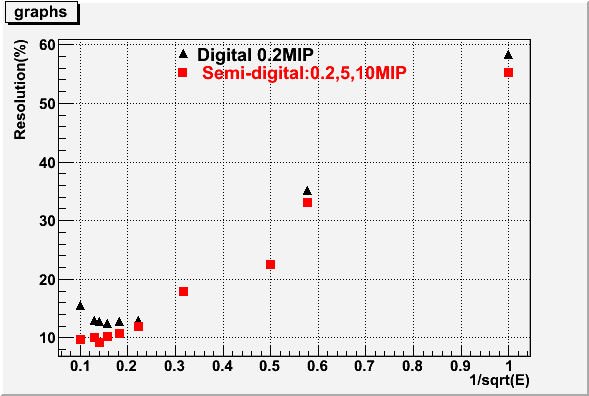
\includegraphics[width=0.9\textwidth]{images/DigitalSemiDigital}}
    \end{column}
  \end{columns}


\end{frame}



\section{Data analysis}
\begin{frame}[shrink=5]{Data storage}
  \begin{block}{Collections}
    Two collections are built and stored in LCIO format
    \begin{itemize}
    \item RU\_XDAQ: a list of  GenericObject (vector of Int) containing raw data from RU 
    \item DHCALRawHits: a collection of RawCalorimeterHits containing all hits seen in hardRocs. Thresholds are encoded in the amplitude, position and time in CellIDs.
    \end{itemize}
    Slow control data are stored as parameters in a new RunHeader when read from the DIFs 
  \end{block}
  \pause 
  \begin{block}{DHCALAnalysis}
    A standalone library handling:
    \begin{itemize}
    \item Creation of LCIO file
    \item handling of RU buffer
    \item Creation of RawCalorimeterHits from raw data
    \item Analysis framework
    \end{itemize}

  \end{block}
\end{frame}

\begin{frame}[shrink=5]{Data analysis}
  \begin{block}{Standalone}
    Using DHCALAnalysis library
    \begin{itemize}
    \item Abstract Analyzers that can be registered (analog to Marlin, no DLL, Factory to be written)
    \item Can be run online
    \end{itemize}
    
  \end{block}
  \pause 
  \begin{block}{Marlin}
    \begin{itemize}
    \item Port of Lyon online analysis
    \item Inclusion in a XDAQ application {\sl MarlinAnalyzer} is done:
      \begin{itemize}
      \item Peformances analog to the standalone version { \sl LCIOAnalyzer}
      \item Possibility to add full reconstruction online 
      \end{itemize}
    \end{itemize}
  \end{block}

\end{frame}


\begin{frame}[shrink=5]{Monitoring}

  \begin{columns}
    \begin{column}{0.5\textwidth}
      \par
      Based on ROOT. Still preliminary. Few tools to handle histograms and display them online.


      \begin{block}{DCHistogramHandler}
        Tool class handling a hashmap of TH1 and TH2 histograms with structured names:
        \par
            {\sl /TOP/DIF21/HitMap ... }
            \begin{itemize}
            \item Direct access on name to the histograms
            \item Query of histograms on regular expressions
            \item Canvas/ Images creation based on those queries
            \item Histograms storage follows the structure
            \end{itemize}


      \end{block}
    \end{column}
    \begin{column}{0.5\textwidth}
      \pause \begin{block}{Toy web interface in LCIO/MarlinAnalyzer}
        \begin{itemize}
        \item CGI handling of regular exp. or of the histogram structure
        \item Canvas creation and display inside web page
        \end{itemize}
      \end{block}

      \centerline{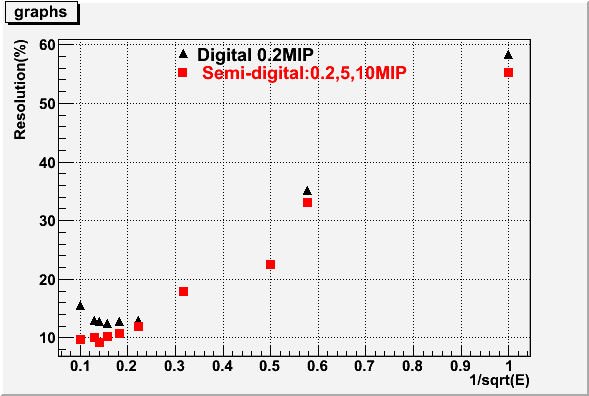
\includegraphics[width=0.9\textwidth]{images/DigitalSemiDigital}}

    \end{column}
  \end{columns}
\end{frame}

\section{Results}
\begin{frame}{Spring 2010 Beam tests}
  \begin{block}{May 2010 (T9 PS)}
    First use of the Event Builder in beam test
    \begin{itemize}
    \item Two $1  m^2$ chambers , 6 DIFs
    \item One additional trigger board (TSC) to control the trigger
    \item First tests with the CCC 
    \end{itemize}
  \end{block}
  \pause \begin{block}{June 2010 (H2 SPS)}
    \begin{itemize}
    \item $1/6 m^2$ chamber ( 1 DIF, 24 HR2)
    \item B= 3 T field
    \item Power pulsing mode
    \item No trigger control anymore
      \begin{itemize}
      \item back pressure from DIF busy signal
      \item hardware veto for EVB overflow 
      \end{itemize}      
    \end{itemize}
  \end{block}
\end{frame}
\begin{frame}{Laboratory tests}
  \begin{block}{Speed}
    \begin{itemize}
    \item The main limitation comes from the USB readout of the hardrocs. Typical readout speed is ~ 500 Hz
    \item More complex analysis can slow down heavily the performances and requires adjustements in the EVB structure and size.
    \end{itemize}
  \end{block}
  \pause
  \begin{block}{Calibrations}
    The EVB structure allows an easy implementation of any calibration loop
    \begin{itemize}
    \item TA block the trigger(veto) and change parameters (Message to DIF)
    \item TA send N trigger with the new params and wait for data collection
    \item Pedestals and HR2 calibration with injection are already implemented 
    \end{itemize}
  \end{block}
\end{frame}

\section{Futur}



\begin{frame}{$ 1 m^3 $ prototype }

  \begin{block}{New Hardware}
    Integration of DCC and LDA in the framework. It should be easy with the use of RUCollector mechanism
  \end{block}
  \begin{block}{Performances}
    Need to define CPU and storage capabilities required
  \end{block}
  \begin{alertblock}{Monitoring}
    Main issue. The current online monitoring is not suited for large system. Recent MARLIN adaptation should allow new developpers to be involved.
  \end{alertblock}


\end{frame}

\begin{frame}[shrink=15]{ Other developments needed}

  \begin{block}{Configuration database}
    A first prototype of a configuration database (MySQL) is being tested. It handles  a versioned set of all DIF and HardROC parameters of a given setup. First usgage during next week H4 beam test. Compulsory for $1 m^3$ prototype.
  \end{block}
  \pause \begin{block}{Condition database}
    Both data taking conditions and errors need to be logged in a Condition database accessible offline. No implementation yet.
  \end{block}

  \pause \begin{block}{Process configuration}
    Currently, the process creation is manual and the application configuration is controlled by the {\sl LocalManager} via SOAP messages. The system is well suited for standalone setup (1 Partition). Larger system will require to use a separate framework (CMS RCMS?) 
  \end{block}

  \pause \begin{block}{Slow Control}
    All slow control application (HV/LV control, environmental probes) are currently standalone. A common framework and an interface to configuration and condition database is needed.
  \end{block}

\end{frame}

\begin{frame}{Summary}
  \begin{block}{Status}
    SDHCAL acquisition software is based on XDAQ framework for data
    collection and MARLIN for online analysis. The event builder of CMS is
    also used for coherent data collection. 
    \par
    The system has been tested both in laboratory test and in 2 beam tests
    this year.
  \end{block}
  \begin{block}{Futur}
    Several developments are on-going to adapt this daq to the $1 ~ m^3$
    scale: LDA \& DCC integration, Configuration DB and monitoring
  \end{block}

  \begin{block}{Try it}
    XDAQ may look complex but it is not a so heavy framework. 
    \par
    Software is available on SVN. We are ready to help new group to adapt
    their DAQ.
  \end{block}
\end{frame}
